\newpage
\chapter*{Simulations}
\addcontentsline{toc}{chapter}{Simulations} 



\section{Baseline study (find better name)}

\hl{Consider relabeling drag length to sliding distance instead.}

\subsection{Friction simulation parameters}

The friction simulation is governed by a set of parameters where some is kept constant while other is varied to gain insight in the frictional properties. These parameters can be categorised into three main categories of different purpose as described in table \ref{tab:param}. 


\begin{table}[H]
  \begin{center}
  \caption{Parameters of the numerical procedure for measuring friction.}
  \label{tab:param}
  \begin{tabular}{ | c | m{8cm}| m{5cm}|} 
    \hline
    Category & Parameter name: description & Category purpose \\ 
    \hline
    Physical & 
    \begin{itemize}
      \item[-] $T$: Temperature for the Langevin thermostat.
      \item[-] $v_{\text{slide}}$ : Sliding speed for the sheet translation.
      \item[-] $K$: Spring constant for the spring force between the virtual atom and the pull blocks responsible for translating the sheet along the substarte. An infinte spring constant is achieved by moving the pull blocks as a rigid body (Lammps: fix move).
      \item[-] Scan angle: The direction for which we translate the sheet.
    \end{itemize} &
    Parameters expected to have a physical effect on the friction properties, which is kept fixed and thus not included in the machine learning input set. 
    \\ \hline
    Measurement & 
    \begin{itemize}
      \item[-] $dt$: Integration timestep.
      \item[-] $t_R$: Relaxtion time before strething.
      \item[-] Pauses between stretch and adding normal force and between dragging the sheet.  
      \item[-] Stretch Speed: How fast to stretch the sheet.
      \item[-] Slide distance: How far to translate the sheet.
      \item[-] Sheet size: Spatial size of the 2D sheet.  
      \item[-] Pull block size: spatial size of the pull blocks.
    \end{itemize} &
    Paramters influecing the simulation dynamics and being representative of the experimental procedure that we are mimicking. These parameters is chosen with the aim of getting stable parameters under small perturbations of the given parameter. 
     \\ \hline
    ML input & 
    \begin{itemize}
      \item[-] Sheet configuration: A binary matrix containing information of which atoms are removed (0) and which is still present (1) in the graphene sheet. 
      \item[-] Stretch amount: The relative sheet stretch in percentage.
      \item[-] $F_N$: Applied normal force to the pull blocks.
    \end{itemize} &
    The remaining paramters serves as input variables for optimization process and is thus given as input variables for the machine learning (ML). 
    \\ \hline
  \end{tabular}
  \end{center}
\end{table}

Due to the great number of parameters, and corresponding range of reasonable numerical values they can take, it is ... to parameter search including all of these. Thus, we will to a great extent rely on a reverse engineering in order to establish a set of parameters for the \textit{physical} and \textit{measurement} categories along with numerical ranges for the $\textit{ML input}$ category which gives stable and promising results. By doing so we effectively narrow down the parameter regime for which the investigated frictional properties belong. We aim to chose the parameters in order to accomodate a balance between generlizable and stable result which is simmutaneously a suting candidate as a proof of concept for the control of friction properties using kirigami inspired cuts. 

In the following we present the results of the friction simulations in parallel to the procedure of investigating the choice of different parameters. 

In the following subsections (X to Y) we are going to present the friction simulation results in parallel to the presentation of the reasoning behind the parameter choices. For this we will refer to the default parameter choice showcased in table \ref{tab:final_param} which is representative of the final parameter choices. 




\begin{table}[H]
  \begin{center}
  \caption{Final parameters for the friction simmulations \hl{Probably not the neatest format for this...}}
  \label{tab:final_param}
  \begin{tabular}{ | m{3cm} | m{3cm}| m{3cm} |} \hline
    Physical & Measurements & ML input \\ \hline
    {\begin{align*}
      T &= \SI{300}{K}  \\
      v_{\text{slide}} &= \SI{20}{m/s}  \\
      K &= \inf \text{(LAMMPS: \textit{fix move})}  \\
      \text{Scan angle} &:  (x,y) = (0,1)  
    \end{align*}} &
    {\begin{align*}
      dt &= \SI{1}{fs} \\
      t_R &= \SI{15}{ps} \\
      \text{Pauses} &= \SI{5}{ps} \\
      \text{Stretch speed} &= \SI{0.01}{ps^{-1}} \\
      \text{Slide distance} &= \SI{400}{Å} \\
      \text{Sheet size} &= 130.029 \times \SI{163.219}{\text{Å}} \\
      \text{Pull block size} &= 2 \times 130.029 \times \SI{15.183}{\text{Å}}
    \end{align*}} &
    {\begin{align*}
      \text{Sheet configuration} &= \text{Contiguous} \\
      \text{Stretch amount} &= \text{Below rupture} \\
      F_N &= [0.1, 10] \ \text{nN}
    \end{align*}}
    \\ \hline
  \end{tabular}
  \end{center}
\end{table}



Say someting about how these parameters is chosen. Reference to articles for which these was mirrored from. 


% Which articles is used as a reference for choosing these variables?


% The sliding velocity is 20 m/s, which is comparable to the operating conditions in micromechanical systems (MEMS), but which is much larger than the typical velocity in scanning force microscopy (SFM) experiments. \cite{mo_friction_2009} Supplementary materials.


% We should try to set the physcis and measurement parameters in such a way that we reduce computation speed where it is doesn't infer with the frictional properties study.

% We need to define some ranges for the ML input paramters. $F_N$, stretch ranges where it is not prone to ruptures. The configuration it self does not have clear rules but is also being regulated by the no rupture requirement. 

% Retardation effects due to the finiteness of the speed of sound are usually irrelevant in slow-speed experiments (v < 1 mm/s) \cite{Manini_2016}

% In macroscopic tribology experiments, sliding speeds often range in the 0.1 − 10 m/s region \cite{Manini_2016}

% By contrast, in nanoscale AFM experiments the tip usually advances at much lower speeds $\sim$ 1 $\mu$m/s: over a typical run it is possible to simulate a tiny ∼ 1 pm displacement, far too small to explore even a single atomic-scale event, let alone averaging over a steady state.\cite{Manini_2016}


% However, MD simulations can provide so much physical insight that they make sense even if carried out at much higher speeds than in real-life AFM or surface force apparatus (SFA) experiments: in practice, currently the sliding speeds of most atomistic tribology simulations are in the $\sim$ 1 m/s region.\cite{Manini_2016}


% Besides the limitations of system size and simulation times that are obvious and will be discussed later, there is another limitation concerning temperature, that is rarely mentioned. All classical frictional simulations, atomistic or otherwise, are only valid at sufficiently high temperature. They become in principle invalid at low temperatures where the mechanical degrees of freedom of solids progressively undergo ”quantum freezing”, and both mechanics and thermodynamics deviate from classical. \cite{Manini_2016}.


\subsubsection{Pressure reference for normal load domain}
\text{Find place to put this.}

% source 1: stiletto heeled shoes with less than 1cm diameter:
% https://www.researchgate.net/publication/342223559_How_the_stiletto_heeled_shoes_which_are_popularly_preferred_by_many_women_affect_balance_and_functional_skills

In order to relate the magntidue of the normal force in our friciton measurement
we will use the pressure as a reference. We will use the pressure underneath a
stiletto shoe as a worst case for human pressure execuation underneath the
shoes. From (source 1) it is reported that the diameter of a stiletto heeled
shoe can be less than 1 cm. Hence a 80 kg man\footnote{Yes, a man can certainly
wear stilleto heels.} standing on one stiletto heel (with all the weight on the
heel) will result in a pressure
\begin{align*}
  P = \frac{F}{A} = \frac{mg}{r^2\pi} = \frac{\SI{80}{kg} \cdot \SI{9.8}{\frac{m}{s^2}}}{(\frac{\SI{1e-2}{m}}{2})^2 \pi} = \SI{9.98}{MPa} \\
\end{align*} 

% source 1:
% https://www.schoolphysics.co.uk/age16-19/Mechanics/Statics/text/Pressure_/index.html
While this is in itself a spectacular realization that is often used in
introductory physics courses (source 2) to demonstrate the rather extreme
pressure under a stiletto heel (greater than the foot of an elephant) (how many
Atmos?) this serves as a reasonible upperbound for human executed pressure. With
a full sheet area of $\sim\SI{21e3}{{\text{Å}}^2}$ we can achieve a similar pressure of
$\sim \SI{10}{MPA}$ with a normal force of
\begin{align*}
  F_N = \SI{10}{MPa} \cdot \SI{21e-17}{m^2} = \SI{2.10}{nN}  
\end{align*}

Of course this pressure might be insufficient for various industrial purposes,
but with no specific procedure in mind this serves as a decent reference point.
Notice that if we consider a human foot with ares $\SI{113}{cm^2}$ the pressure
drops to a mere $\SI{70}{kPa}$ corresponding to $\sim \SI{0.01}{nN}$.

% source 3: foot area ≈ 113 cm^2:
% https://www.footbionics.com/Patients/Foot+Facts.html source 4:
% https://hypertextbook.com/facts/2003/JackGreen.shtml




\newpage
\subsection{Single friction simulation analysis}\label{sec:single_analysis}
We begin by assessing the raw data for a single friction simulation run with the default parameters shown in table \ref{tab:final_param} for a non-cut sheet, no stretch and an applied normal force of $\SI{1}{nN}$.


\subsubsection{Force oscillations}\label{sec:force_oscillations}
We first assess the raw data for the friction force $F_{\parallel}$ parallel to the drag direction as seen in figure \ref{fig:drag_Ff}. The sample rate is 10 ps$^{-1}$ = 100 timesteps$^{-1}$ for which each sample is the mean value of the 100 timesteps preceding the given sample interval. We observe immediately that the data carriers oscillations on different time scales. By applying a savgol filter to the data with a polyorder of 5 and window length of 150 timesteps, corresponding to a sliding distance of 3 Å or a time window of 15 ps, we can qualitatively point out at least two different frequencies of osccilation. On figure \ref{fig:drag_Ff_10} we see roughly three waves on the savgol filter corresponding to a relative high frequency, while on \ref{fig:drag_Ff_100} the same savgol filter reveals a lower frequency on top of the first, creating the visual pattern of a wavepacket.

\begin{figure}[H]
  \centering
  \begin{subfigure}[t]{0.49\textwidth}
      \centering
      \includegraphics[width=\textwidth]{figures/baseline/drag_Ff_10Å.pdf}
      \caption{Drag length of 10 Å.}
      \label{fig:drag_Ff_10}
  \end{subfigure}
  \hfill
  \begin{subfigure}[t]{0.49\textwidth}
      \centering
      \includegraphics[width=\textwidth]{figures/baseline/drag_Ff_100Å.pdf}
      \caption{Drag length of 100 Å.}
      \label{fig:drag_Ff_100}
  \end{subfigure}
  \hfill
     \caption{Friction force $F_\parallel$ with respect to the drag direction between (full) sheet and substrate versus sliding distance. The sliding distance is measured by the constant movement of the virtual atom and not the COM of the sheet. However, we expect these measures to be fairly identical due the fact that the pull blocks is rigidly coupled to the virtual atom. The red line represents a savgol filter with window polyorder 5 and window length of 150 timesteps (corresponding to a sliding distance of 3 Å or a time window of 15 ps).}
     \label{fig:drag_Ff}
\end{figure}

By performing a Fourier Transform (FT) on the data we can quantify the leading frequencies as seen in figure \ref{fig:ft_a}. By plotting the two most dominant frequencies $f_1 = 0.0074$ ps$^{-1}$ and $f_2 = 0.0079$ ps$^{-1}$ as $\sin{(2\pi f_1)} + \sin{(2\pi f_2)}$ we find a qualitatively convincing fit to the observed wavepacket shape as seen in figure \ref{fig:ft_b}. By using the trigonometric identity
\begin{align*}
\sin (\alpha+\beta) &= \sin (\alpha) \cos (\beta) + \cos (\alpha) \sin (\beta), \\
\sin (\alpha-\beta) &= \sin (\alpha) \cos (\beta) - \cos (\alpha) \sin (\beta),
\end{align*}
and decomposing $f_1 = a - b$, $f_2 = a + b$ we can rewrite the sine sum as the sinusoidal product
\begin{align*}
  \sin(2\pi f_1) \sin(2\pi f_2) &= \sin\big(2\pi (a - b)\big) \sin\big(2\pi (a + b)\big) \\
  &= \sin(a)\cos(b) + \cancel{\cos(2\pi a)\sin(2\pi b)} + \sin(2\pi a)\cos(2\pi b) - \cancel{\cos(2\pi a)\sin(2\pi b)} \\
  &= 2 \sin(2\pi a) \cos(2\pi b),
\end{align*} 

with 
\begin{align*}
  a = \frac{f_1 + f_2}{2} &= 0.0763 \pm \SI{0.0005}{ps^{-1}},& 
  b = \frac{f_2 - f_1}{2} &= 0.0028 \pm \SI{0.0005}{ps^{-1}},& \\
  &= 0.381 \pm \SI{0.003}{{\text{Å}}^{-1}},& 
  &= 0.014 \pm \SI{0.003}{{\text{Å}}^{-1}},& 
\end{align*}
where the latter frequency is denoted with respect to the sliding distance. This makes us recognize the high osccilation frequency as $a$ and the low frequency as $b$. The faster one has a period of $T_a = 2.62 \pm 0.02$ Å\footnote{The uncertainty $\Delta y$ is calculated as $\Delta y = \left|\frac{\partial y}{\partial x} \Delta x \right|$ for uncertainty $\Delta x$ and $y(x)$}. This corresponds well with the magnitude of the lattice spacing and especialy that of graphene at 2.46 Å as expected theoretically (make reference to theory section?). We also take note of the longest period $T_b = 71 \pm 15$ Å$^{-1}$ which will be relevant for the evaluation of measurement uncertainty in section \ref{sec:def_dyn_and_stat}.

\begin{figure}[H]
  \centering
  \begin{subfigure}[t]{0.49\textwidth}
    \centering
    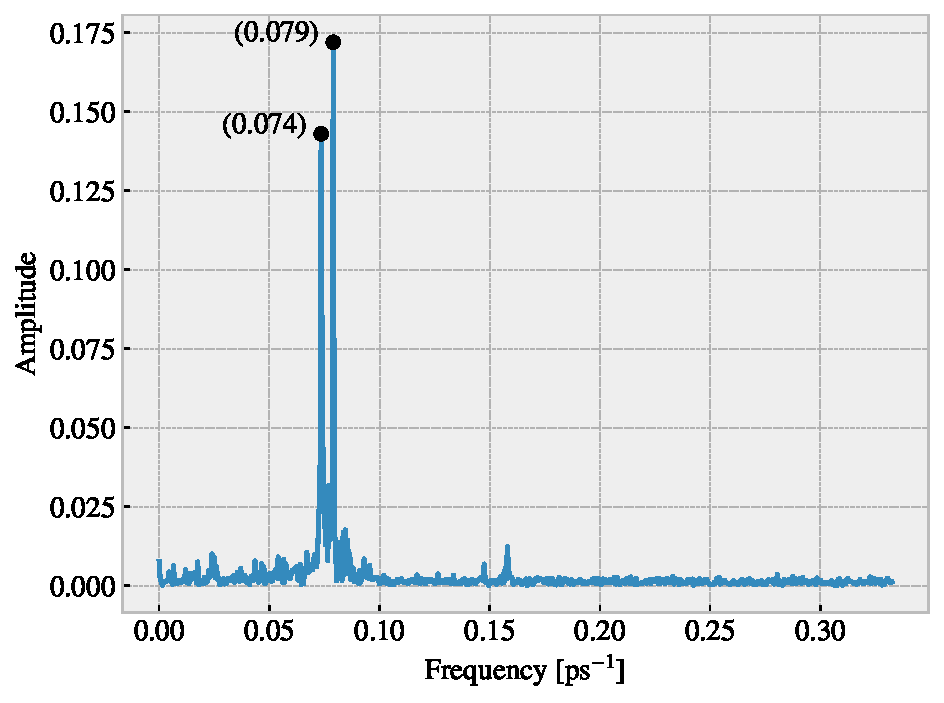
\includegraphics[width=\textwidth]{figures/baseline/ft_zoom.pdf}
    \caption{FT result shown for a reduced frequency range.}
    \label{fig:ft_a}
  \end{subfigure}
  \hfill
  \begin{subfigure}[t]{0.49\textwidth}
      \centering
      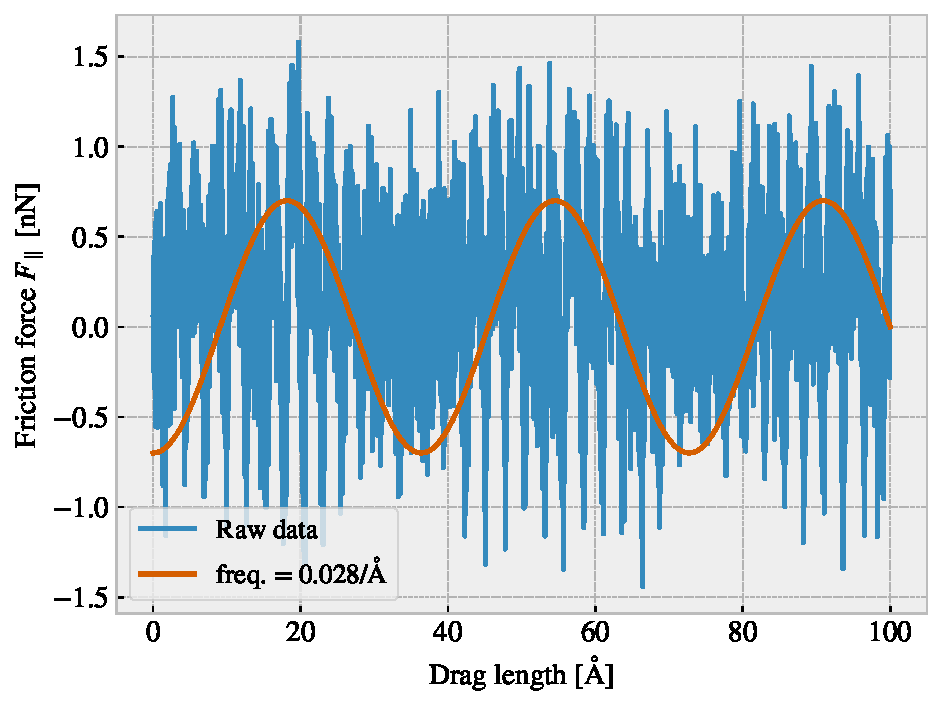
\includegraphics[width=\textwidth]{figures/baseline/ft_sine.pdf}
      \caption{Two most dominant frequencies applied to the data from figure \ref{fig:drag_Ff_100}}
      \label{fig:ft_b}
  \end{subfigure}
  \caption{Fourier transform (FT) analysis of the full friction force data (all 400 Å sliding distance) shown in figure \ref{fig:drag_Ff}. (a) shows the two most dominant frequency peaks. Note that no significant peaks was found in a higher frequency than included here. (b) shows a comparison between the raw data and the wavefunction corresponding to the two peaks in figure (a).}
  \label{fig:ft}
\end{figure}


\subsubsection{Decompositions}
In the previous analysis we have looked only at the friction force for the full
sheet, including the pull blocks which is locked off during sliding, and with
respect to the drag direction. This represents our choice measurement which we will adress in the following.

Due to the fact that we are only applying cuts to the inner sheet (excluding the
pull blocks), it might seem more natural to only consider the friction on that
part. If the desired frictional properties can be achieved by altering the inner
sheet one can argue that any opposing effects from the pull blocks can be
mitigated by scaling the relative size between the inner sheet and the pull
blocks. However, when looking at the time series of the friction force
decomposed with respect to the inner sheet and pull block region (see figure
\ref{fig:decomp_group}), we observe the friction force arrising from those parts
are seemingly antisymmetric. That is, the distribution of the fricitonal pull from the substrate on the sheet is
oscillating between the inner sheet and the pull block. Keeping in mind that 
normal force is only applied to the pull blocks we might take this as an
integrated feature of the system which does not nessecary dissapear when changing the spatial ratio between inner sheet and pull block. Any interesting friciton properties might depend on this internal distribution of forces. Hence, we hedge our bets
and use the full sheet friction force as a hollistic approach to this measurement
problem.

Similar we might question the decision of
only considering the frictional force projected onto the sliding direction as
we are neglecting the ``side shift'' induced during the slide phase. In figure \ref{fig:decomp_direc} we see the decomposition into force components parallel $F_{\parallel}$ and perpendicular $F_{\perp}$ to the slide direction respectively. We see that the most dominant trends is projected into the parallel component. If we want to include the perpendicular component as well we would have to evaluate the friction as the length of the force vector for which we would lose the sign of the force direction. Hence, we would only get a positive contributin which would not be able to capture the change between resisting and assisting the sliding during stick-slip motion. One option to accommodate this is by using the vector length but keeping the sign from the projection parallel to the sliding direction. However, we omit such compromises as this might make analysis interpration more difficult, and we use only the parallel component going forward. 

\begin{figure}[H]
  \centering
  \begin{subfigure}[t]{0.49\textwidth}
    \centering
    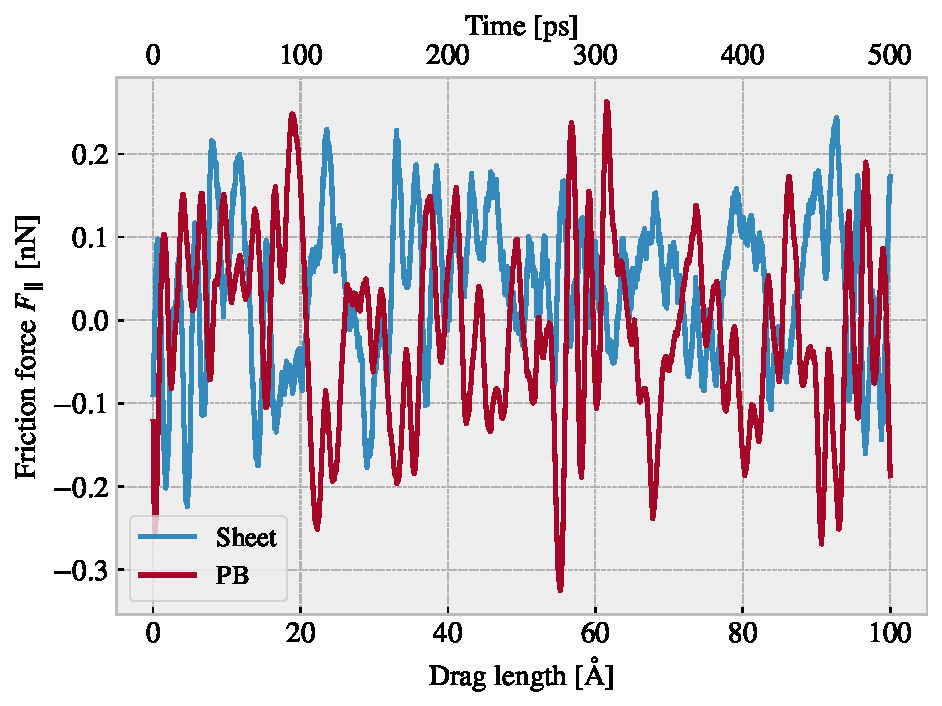
\includegraphics[width=\textwidth]{figures/baseline/decomp_group.pdf}
    \caption{Decomposition into group inner sheet (sheet) and pull blocks (PB).}
    \label{fig:decomp_group}
  \end{subfigure}
  \hfill
  \begin{subfigure}[t]{0.49\textwidth}
      \centering
      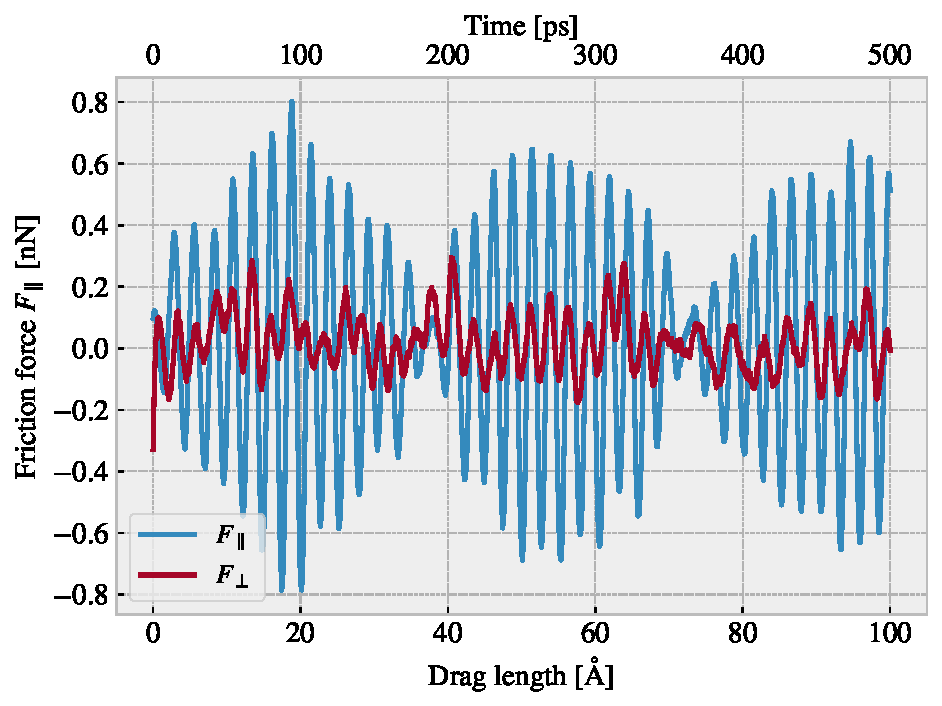
\includegraphics[width=\textwidth]{figures/baseline/decomp_direc.pdf}
      \caption{Decomposition into parallel ($F_{\parallel}$) and perpendicular ($F_{\perp})$ to drag sliding direction.}
      \label{fig:decomp_direc}
  \end{subfigure}
  \caption{Friction force decomposition on the data shown in figure \ref{fig:drag_Ff} with applied savgol filters similar to that of figure \ref{fig:drag_Ff_100} with window polyorder 5 and window length of 150 timesteps (corresponding to a sliding distance of 3 Å or a time window of 15 ps).}
  \label{fig:decomp}
\end{figure}


\subsubsection{Center of mass path}
From the previous observations of the friction force time series we see evidence
of a stick-slip behvaiour. Specially, we see in figure \ref{fig:decomp_direc}
that this might be the case both parallel and perpendicular to the sliding
direction. By looking at the $x,y$-position for the sheet center of mass (COM)
we observe the stick-slip motion manifested as a variation in COM speed combinned
with a side to side motion as shown in figure $\ref{fig:COM_path_K0}$. In an attempt to increase the magnitude of the slips we evaluate a similar simulation with spring contant $K = \SI{30}{N/m}$ (see figure
\ref{fig:COM_path_K30}) in contrast to that of an infinte spring constant. While
the maximum slip speed stays within a similar order of magnitude the slip length
in the sliding direction is increased along with the side to side motion. Note
that the axis scale is different between figure \ref{fig:COM_path_K0} and
\ref{fig:COM_path_K0}. However, in both cases we observe that the side to side
motion is associated with a low speed, meaning that is more reminiscent of a ``slow'' creep alignment with the substrate than a slip. 


\begin{figure}[H]
  \centering
  \begin{subfigure}[t]{0.85\textwidth}
    \centering
    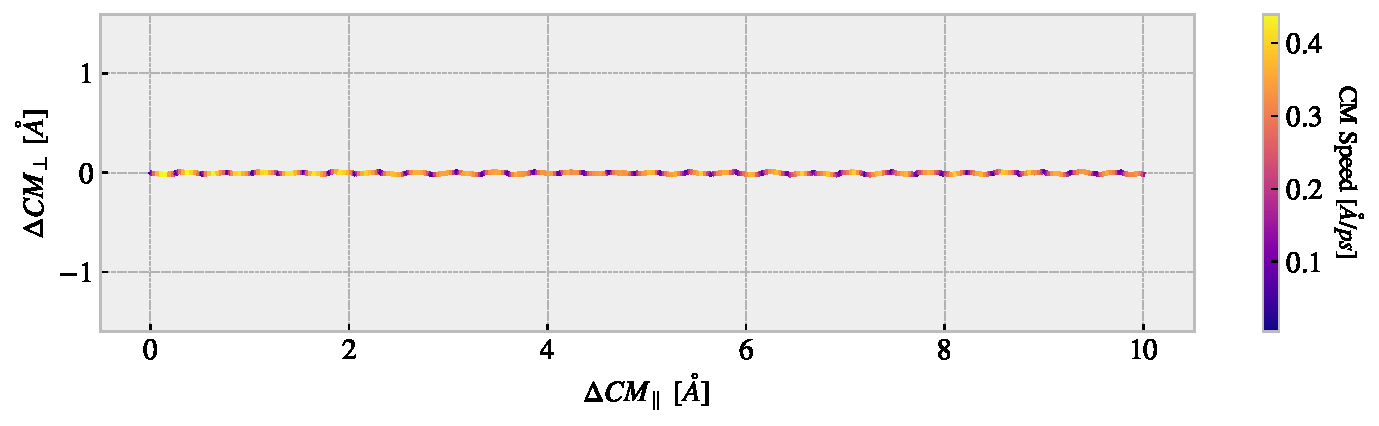
\includegraphics[width=\textwidth]{figures/baseline/COM_path_K0.pdf}
    \caption{$K=\inf$ (Fix move)}
    \label{fig:COM_path_K0}
  \end{subfigure}
  \hfill
  \begin{subfigure}[t]{0.85\textwidth}
      \centering
      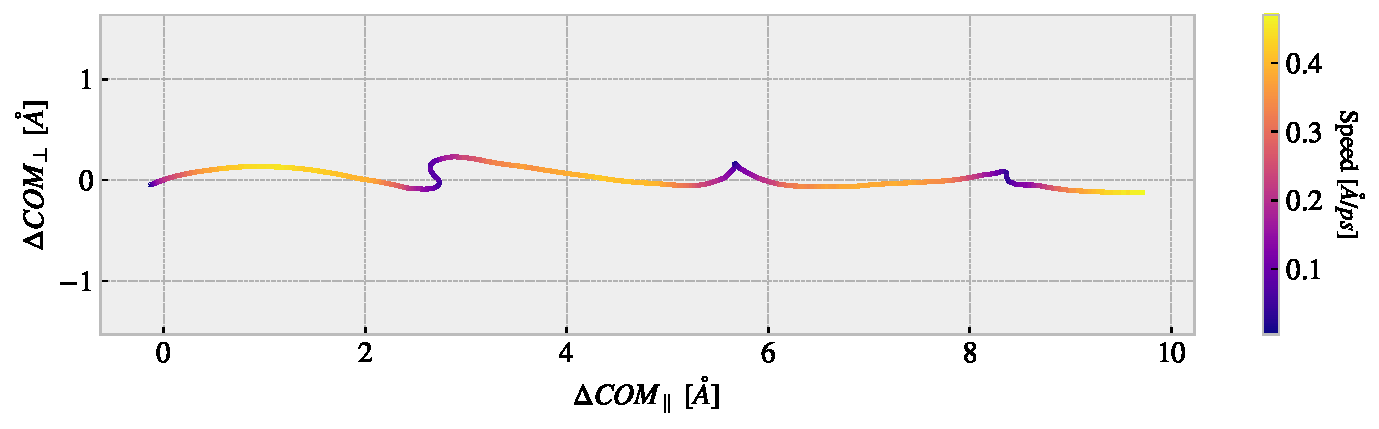
\includegraphics[width=\textwidth]{figures/baseline/COM_path_K30.pdf}
      \caption{$\SI{30}{N/m}$}
      \label{fig:COM_path_K30}
  \end{subfigure}
  \caption{Center of mass posotion relative to the start of the sliding phase in terms of the direction parallel to the sliding direction $\Delta COM_{\parallel}$ and the axis perpendicular to the sliding direction $\Delta COM_{\perp}$. The colorbar denotes the absolute speed of the COM.}
  \label{fig:COM_path}
\end{figure}


\subsection{Defining metrics for dynamic and static friction}\label{sec:def_dyn_and_stat}

In order to evaluate the frictional properties of the sheet we reduce the comprehensive friction force time series adressed in section \ref{sec:single_analysis} into single metrics describing the dynamic and static friciton. The natural choice is to use the mean and max values of the time series. 

\subsubsection{Dynamic friction} 
For the dynamic friction measurement we take the mean value of the latter half
of the dataset to ensure that we are sample from a stable system. For a full
sliding simulation of 400 Å we thus base our mean value on the latter 200 Å of
sliding. In figure \ref{fig:runmean} we have shown the friction force of the
first 10 Å of sliding together with a running mean with window length of 5 Å
corresponding to 50\% the data length. This is merely done to illustrate the
samplig procedure and by only using a 10 Å sliding distance the final mean
estimate (indicated with a dot) takes a negative value due to the specific cut-off of the
few oscialltion captured here. Nonetheless, one approach to quanity the
uncertainy of the final mean estimate is to consider the variation of the
running mean preceeding the final mean value. The more the running mean
fluctuates the more uncertainty associated with the final estimate. However, only the
running mean ``close'' to the ending should be considered, since the first part
will rely on data from the beginning of the simulation. From the Fourier analyse
in section \ref{sec:force_oscillations} we found the longest significant
oscillation period to be $\sim 71$ Å$^{-1}$ corresponding to $\sim 35 \%$ of the
running mean window consisting of 200 Å of slifing when including all the data.  Hence, we use the standard deviation of the final 35\% of the running mean to approximate the
uncertainty of the final mean value, and we estimate the relative error by
dividing the standard deviation by the final mean value. In figure \ref{fig:runstd} we showcase a running standard deviation of a window length $35 \%$ the running mean window in figure \ref{fig:runmean} for the illustrative case of a total 10 Å slide. The final uncertainty value is marked by a dot, and we see as expected that we get a high relative error of $\sim 257\%$ which corresponds well with the short sampling period and the mean value taking an unphysical negative value. 


\begin{figure}[H]
  \centering
  \begin{subfigure}[t]{0.49\textwidth}
    \centering
    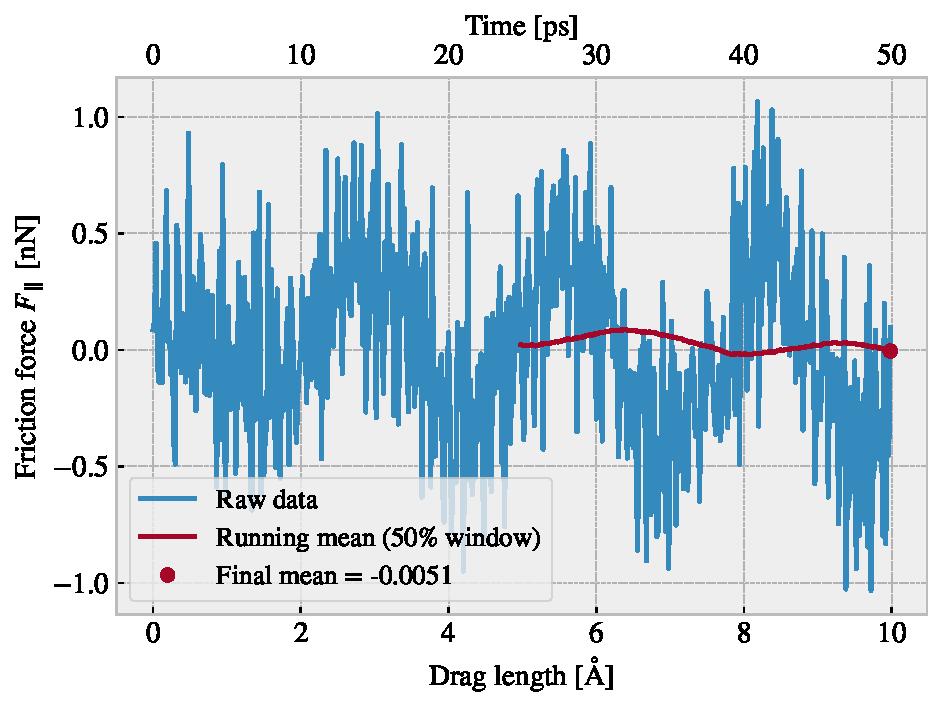
\includegraphics[width=\textwidth]{figures/baseline/Ff_runmean.pdf}
    \caption{Running mean with window length $\SI{5}{\text{Å}}$ (50\% the data length).}
    \label{fig:runmean}
  \end{subfigure}
  \hfill
  \begin{subfigure}[t]{0.49\textwidth}
      \centering
      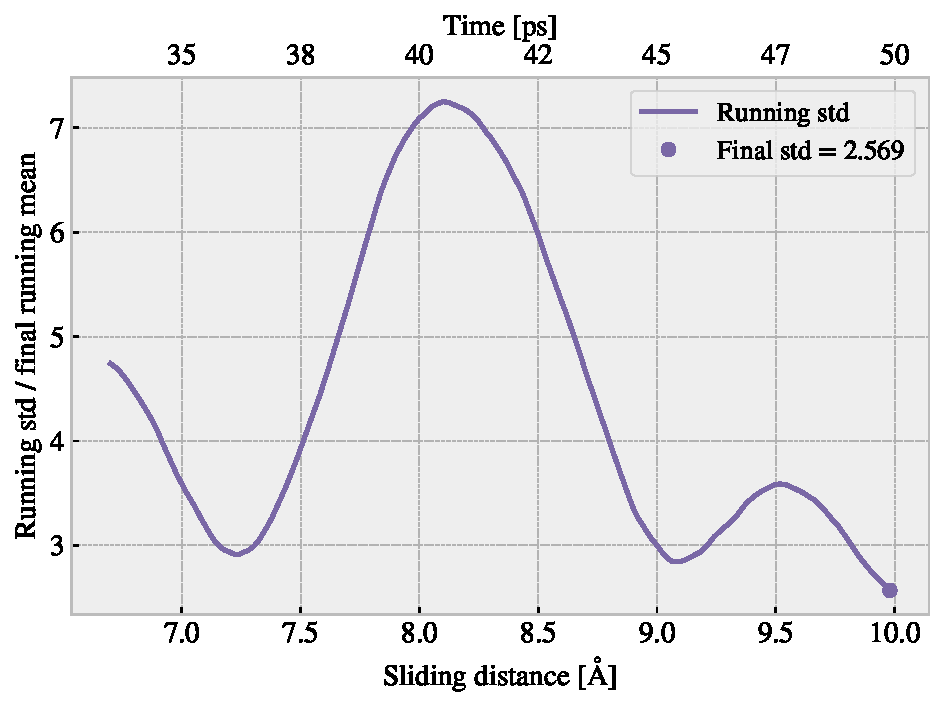
\includegraphics[width=\textwidth]{figures/baseline/Ff_runstd.pdf}
      \caption{Running std with window length $\SI{1.75}{\text{Å}}$ (35\% the mean window length.)}
      \label{fig:runstd}
  \end{subfigure}
  \caption{Running mean and running standard deviation (std) on the friction force data from a $\SI{10}{{\text{Å}}}$ of sliding simulation. The running mean window is 50\% the data length while the running std window is 35\% the running mean window length.}
  \label{fig:running}
\end{figure}


When including the full dataset of 400 Å of sliding, such that std window actually matches with the longest period of oscillations expected from the data, we get a final relative error of $\sim 12 \%$ as shown in fig \ref{fig:runstd_long}. This is arguable just at the limit for an acceptable error, but as we shall see later (\hl{Make a reference to fig or sec}) this high relative error is mainly connected to the cases of low friction. When changing the simulation parameters, such that the mean friction evaluates to considerable higher values, the relative error drops to the order (\hl{put in numbers}). One interpration of this finding is simply that the oscialltiosn in the running mean is somewhat independent of the magnitude of the friction. In that case, the relative error will spike for the low friction cases. 


\begin{figure}[H]
  \centering
  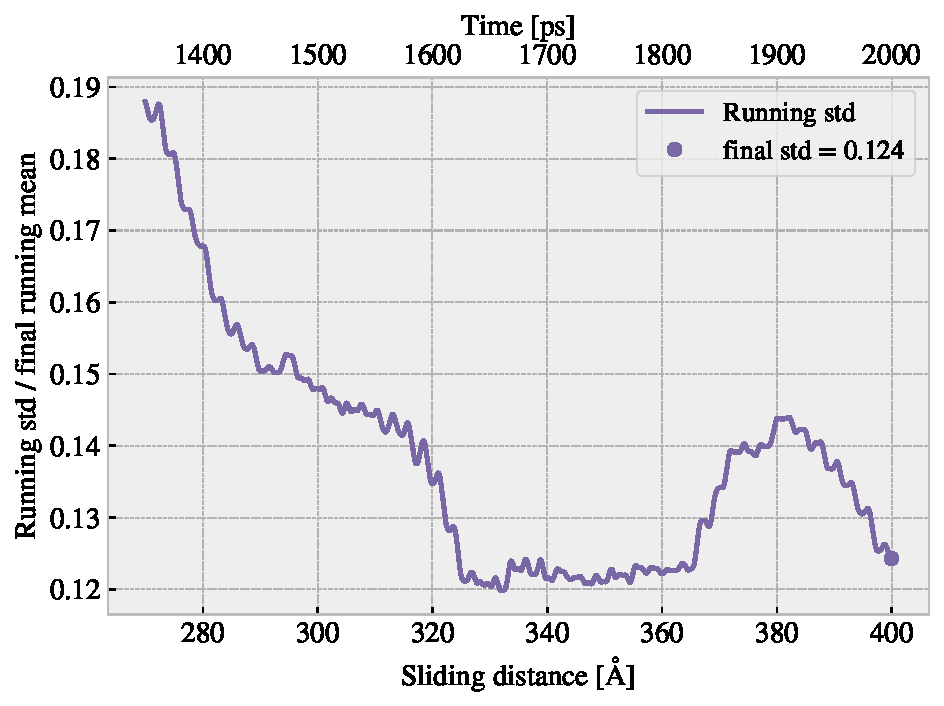
\includegraphics[width=0.6\linewidth]{figures/baseline/Ff_runstd_long.pdf}
  \caption{Running standard deviation (std) for a full \SI{400}{{\text{Å}}} sliding simulation. The running std window is 70 Å (35\% the running mean window of 50\% the data length).}
  \label{fig:runstd_long}
\end{figure}


\subsubsection{Static friction} 
The max value is the most obvious choice for adressing the static friction, even
though that the definition of the static friction is a bit vague. When
considering the friction force time series in figure \ref{fig:drag_Ff} we
observe that the stick-slip oscillations increase in magnitude toward a global
peak at $\sim \SI{20}{\text{Å}}$. Thus, we could identify this peak as the
static friction force, but the global max does in fact rarely fall within the
first part of the sliding. In figure \ref{fig:max_dist} we investigate the top
three max value, at which sliding distance they accour and at what magnitude,
for 30 uniformly sampled normal forces in the interval $[0.1, 10]$ nN. It is
immediately clear that only few of the peaks falls within the ``beginning'' of
the simulation defined by the slowest significant oscialltion period of $71\pm
\SI{15}{\text{Å}}$. In fact only 2/30 global values and 4/90 top three values
can be associated to the start of the sliding by this definition. Thus, this
result suggest that the max value cannot be used as a reliable measure for the
static friction either due to its lack of presence or due to the simulation
setup procedure. For a more typycal evaluation of the static friction force one
would increase force slowly until the first slip significant slip is recorded (a
series of precursors is expected to precede this). In our simulations we drag
the sheet relatively fast in a rigid manner which might be the reason for the lacking the static friction. Bonelli et al.\ \cite{bonelli_atomistic_2009} reported that the stick-slip behaviour was only presented when using a relatively soft spring. Thus, by changing the spring constant we investigate possibility to observe a static friction (\hl{I kind of interchanged stick-slip and static friction int his argument, but I still think it can be used to argue for doing the test...}) response within the framework of our simulation procedure as shown in
figure \ref{fig:max_vs_K}. However, the results do not indicate any implications
that a recognizable domain exist for which the static friction response would be
reliable. Hence, we will base the final assesment on frictional properties
purely on the dynamic friction force. 


\begin{figure}
  \centering
  \begin{minipage}[t]{.47\textwidth}
    \centering
    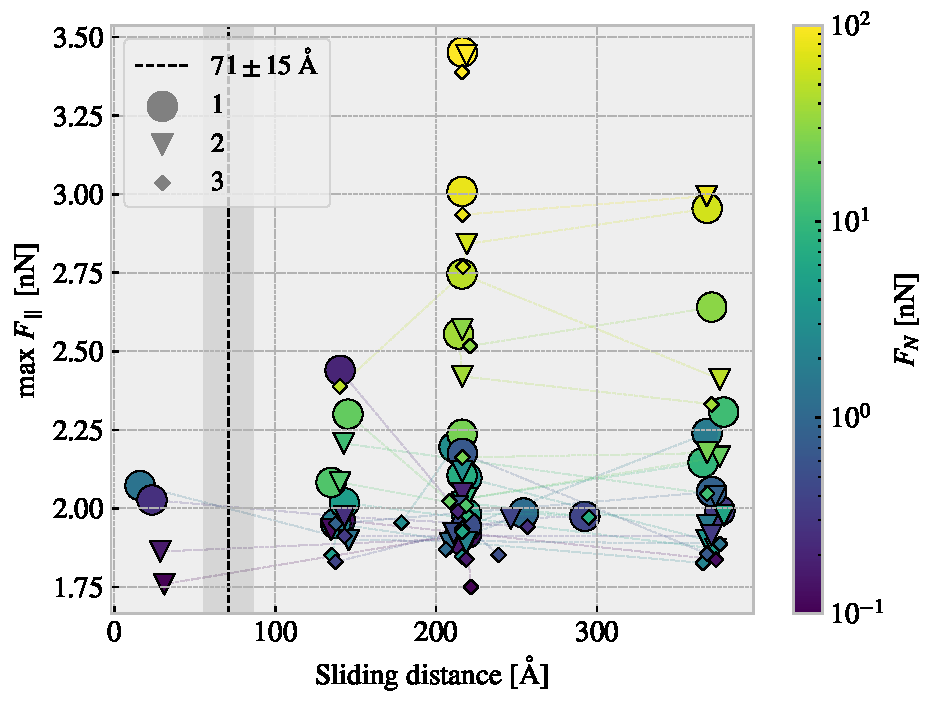
\includegraphics[width=\linewidth]{figures/baseline/max_dist.pdf}
    \captionof{figure}{Distribution of top three max friction force peaks for 30 uniformly sampled normal forces $F_N \in [0.1, 10]$ nN. The dotted line and the grey area marks the slowest significant oscialltion period found in the data and thus marking a dividing line for whether a peak falls within the ``beginning'' of the sliding simulation.}
    \label{fig:max_dist}
  \end{minipage}%
  \hspace{0.2cm}
  \begin{minipage}[t]{.48\textwidth}
    \centering
    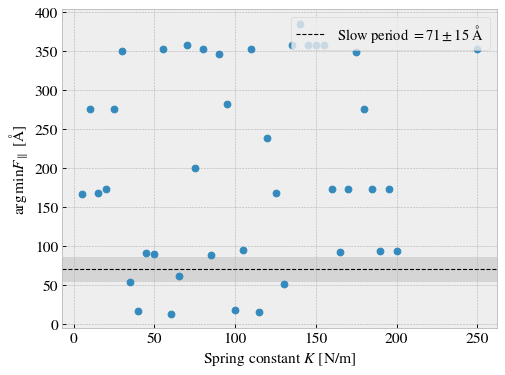
\includegraphics[width=\linewidth]{figures/baseline/max_vs_K}
    \captionof{figure}{Sliding displacement for the max friction peak to appear as a function of spring constant. \hl{Fixmove is tmp mapped to K = 200 here without any discontinuous lines.}}
    \label{fig:max_vs_K}
  \end{minipage}
  \end{figure}




% We investigate the placement of the max values, i.e. the sliding distance length for which we measure the max friction force. We show the placement of the top three max values for different simulatiosn with varying normal force in figure \ref{fig:max_dist}. We observe immediately that only a few top three max values is measured within a full slow period of $\sim$ 71 Å. In fact many max values is measured just before the end of the simulation. This indicates that the naive approach of using the overall max value to describe the static friction coefficient might be a to naive approach. Another approach is to use the max value within a single period, but we do not really know if this period will be similar for alle cut patterns and thus this might be limiting. 



% Look into static friction when having a spring connected to the drag force with
% rather low spring constant. Maybe compare to critical sitffness in FK model.
% Some rough calculations follow here (make a note about this being a very naive
% approach to determine a suitable stiffness for static friction scenarious. In
% reality one should increase force slowly to observe this probably). When
% dragging the sheet in the y-direction we effectively have a lattice spacing
% \begin{align*}
%   a_c = a_{2,x} + B_x = a_G\frac{\sqrt{3}}{2} + \frac{a_G}{2\sqrt{3}} = \frac{2a_G}{\sqrt{3}}
% \end{align*}
% for graphene lattice constant $a_G = 2.46$ Å. For the diamond silicon structure
% this is essentially equal to the lattice constant $a_D = 5.4210$ Å. This gives 
% \begin{align*}
%   \theta = \frac{a_c}{a_b} = \frac{2}{\sqrt{3}}\frac{a_G}{a_D} \approx 0.5230.
% \end{align*}
% Since we have the factor $2/\sqrt{3}$ it is safe to assume that this is a
% irrational number leadning to incommensurability. The worst case scnario of
% incommensurability (where $\theta$ equals the golden-mean, Can we get the exact
% number?) gives the minimal critical stiffness $K_c \sim 2U_0
% (\frac{\pi}{a_b})^2$, where $U_0$ is the substrate potentiual magnitude and
% $a_b$ the lattice spacing of the substrate. The potential barrier $U_0$ can be
% approximated by the work done when resisting the normal force as $\sim F_N
% a_D/2$ such that the critical stiffness can be approximated to 
% \begin{align*}
%   K_c \sim 2 F_N \frac{a_D}{2} \left(\frac{\pi}{a_D}\right)^2 = \frac{F_N}{a_D}\pi^2
% \end{align*}
% With a normal force of 1 nN we get $K_c \sim 18$ N/m. Hence, we should try a
% spring constant lower than that as qualified way of determining if this is the
% reason why we do not really see static friciton in the simulation. By plotting the max position (in terms of drag length) as a function of spring constant as seen in figure \ref{fig:max_vs_K} we can investigate if the concept of a critical spring constant is governing this simulation. However, as I'm writing this I'm realizing that the spring constant in the model applies to the interatomic forces and not the one dragging the system.....




\subsection{Out of plane buckling}

The out of plane buckling is the main motivation for applying the kirigami
inspired cuts to the sheet. Thus, we perform a stretch simulation in a low
temperature $T = \SI{5}{K}$ vacuum in order to verify that the chosen cut
configurations do in fact contribute to a significant out of plane buckling when
stretched. For the non-cut, popup and honeycomb configuration we assess the
movement in the z-direction (perpendicular to the plane) during the stretch,
which we visualize by the min and max z-value along with the atom count
quartiles 1\%, 10\%, 25\%, 50\% (median), 75\%, 90\% and 99\% as shown in figure
\ref{fig:buckling_quartiles}. We observe that the popup and honeycomb pattern
buckles considerable out of plane during the stretch in comparison to the non-cut sheet which only exhibit minor buckling of $\sim 2$ Å which is on the same order as the
atomic spacing in the sheet. We also notice that the popup pattern
buckles more in consideration to the min and max peaks while the 1\%, 99\%
quartiles is on the same magnitude as the honeycomb. By looking at the simulation visualization
(\hl{include OVITO figures for vacuum stretch as well?}) we can conclude that this is mainly due to the fringes
of the sheet ``flapping'' around. 


\begin{figure}[H]
  \centering
  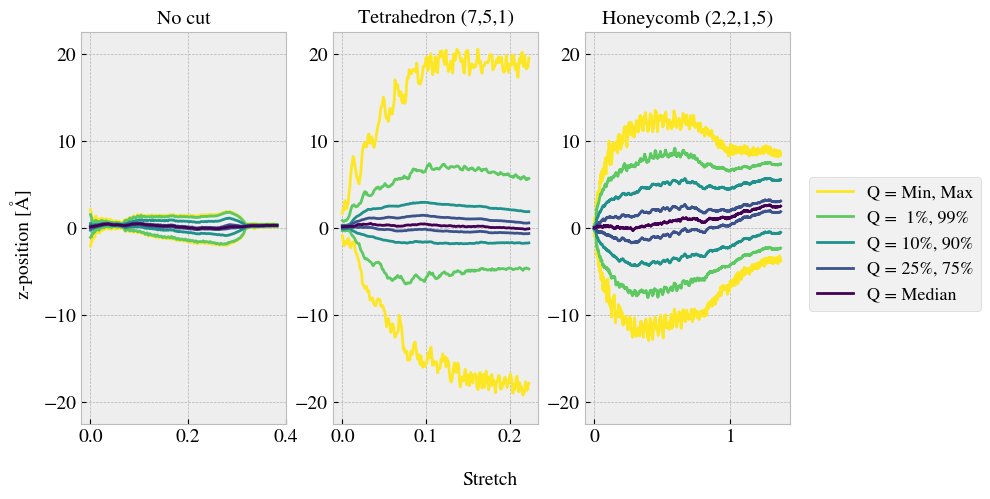
\includegraphics[width=\linewidth]{figures/baseline/vacuum_normal_buckling}
  \caption{Out of plane buckling during stretch of sheets in vacuum at $T = 5$ K. Reading from left to right the vacuum rupture stretch are 0.38, 0.22 and 1.37. \hl{perhaps use a color scale instead of the standard color cycles here.}}
  \label{fig:buckling_quartiles}
\end{figure}


The next step is to verify that the buckling will lead to a significant altering
of the contact area when the sheet is in put in contact with the substrate. We
investigate this by simulating the stretch at the default temperature $T =
\SI{300}{K}$ with the presence of contact forces between the sheet and
substrate. Note that no normal load is applied as the sheet and substrate is
sufficiently attracted by the LJ potential. Selected frames from the simulation is shown in appendix \ref{sec:sheet_stretch}. We assess the contact area by the
relative amount of atoms in the sheet within chemical range of the substrate.
The cut-off for this interaction is 4 Å corresponding to $\sim 120$\% the LJ
equilibrium distance. Since the contact area is usually calculated as the amount
of atoms in contact multiplied with an associated area for each contact this
feature is taken to be proportional to the contact area. The relative amount of
bonds as a function of stretch for the various configurations is shown in figure
\ref{fig:contact_vs_stretch} which clearly indicates a drop in contact area as
the cutted sheets are stretched. 

\begin{figure}[H]
  \centering
  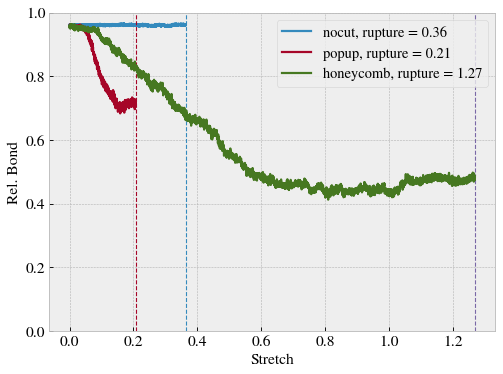
\includegraphics[width=0.6\linewidth]{figures/baseline/contact_vs_stretch.png}
  \caption{Contact vs. stretching of the sheet, where the contact is measured by the relative amount atoms in the sheet within chemical interaction range to the substrate. The cut-off for this interaction range is 4 Å corresponding to $\sim 120 \%$ the LJ equilibrium distance. $T = 300$ K }
  \label{fig:contact_vs_stretch}
\end{figure}

\hl{Compare figure} \ref{fig:contact_vs_stretch} \hl{to that of figure} \ref{fig:multi_stretch_contact} \hl{where multiple simulations constitute the stretch-contact curve.}


\subsection{Investigating selected parmeters}

We investigate the importance of the physical variables $T$, $v_{\text{slide}}$ and $K$ (\hl{make plots for scan angle as well?}) and the choice of timestep $dt$. This is done partly understand how the dependencies relate to theoretical, numerical and experimerimental results, and partly to understand how these parameter choices defines the regime for our multi configurational search. We use the default parameters in table \ref{tab:final_param} with exception of the single parameter of interest which is varied in a reasonable range of the default choice. In figure \ref{fig:var_temp}-\ref{fig:var_dt} the dynamic friction estimate and the max friction force is shown as a function of $T$, $v_{\text{slide}}$, $K$ and $dt$ respectively. For the dynamic friction estimate the absolute error is denoted by a shaded error which linearly connects the points.


\begin{figure}[H]
  \centering
  \begin{subfigure}[t]{0.49\textwidth}
      \centering
      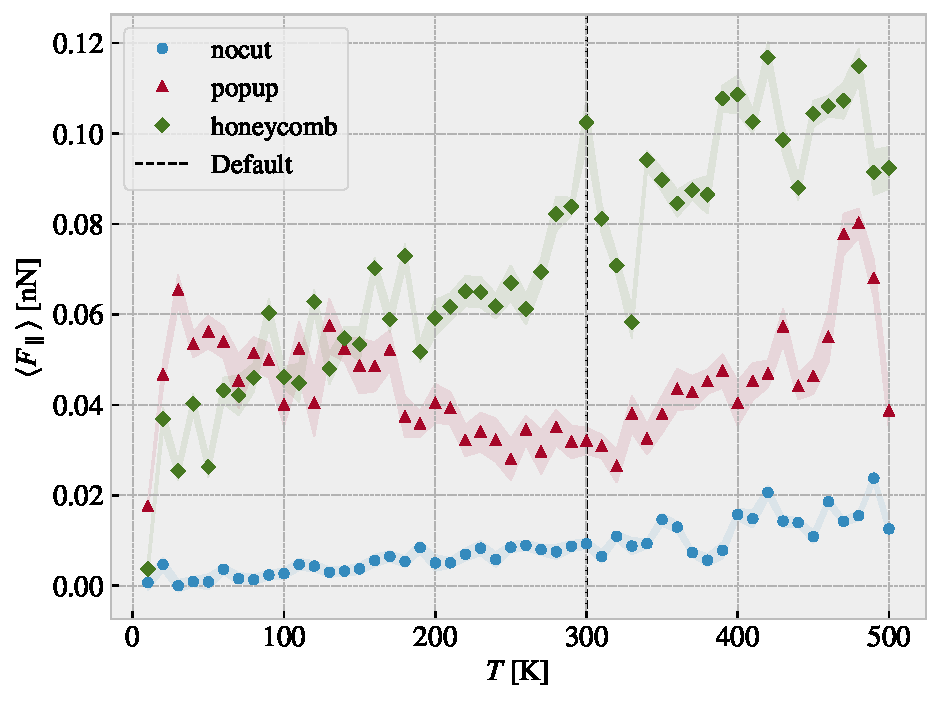
\includegraphics[width=\textwidth]{figures/baseline/variables_temp_mean_fixmove_v20.pdf}
      \caption{Dynamic friction force estimate.}
      \label{fig:var_temp_mean}
  \end{subfigure}
  \hfill
  \begin{subfigure}[t]{0.49\textwidth}
      \centering
      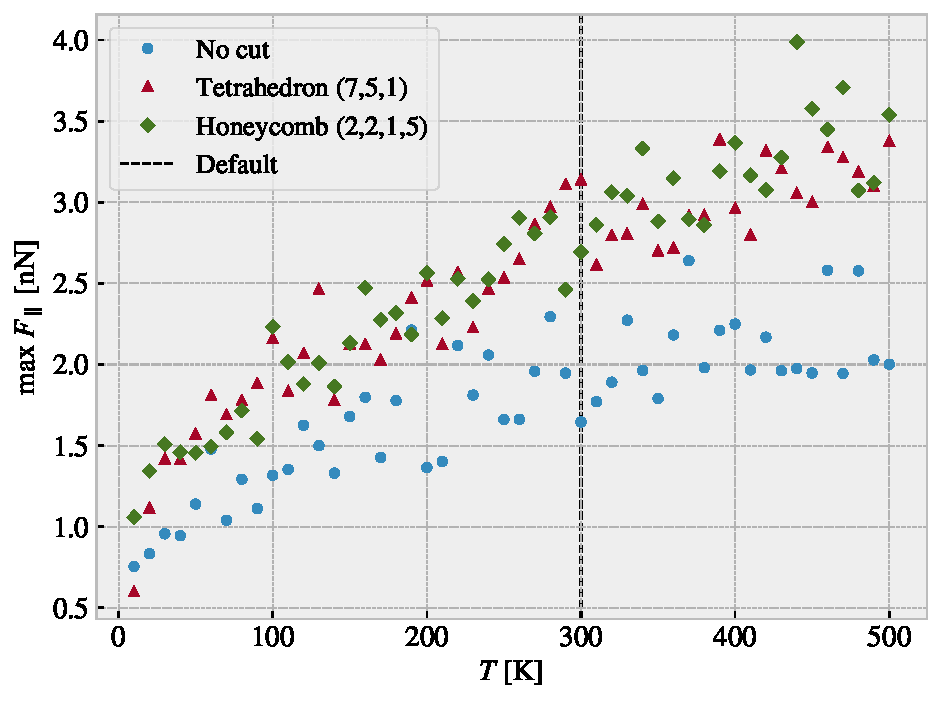
\includegraphics[width=\textwidth]{figures/baseline/variables_temp_max_fixmove_v20.pdf}
      \caption{Max friction}
      \label{fig:var_temp_max}
  \end{subfigure}
  \hfill
     \caption{Temperature.}
     \label{fig:var_temp}
\end{figure}



\begin{figure}[H]
  \centering
  \begin{subfigure}[t]{0.49\textwidth}
      \centering
      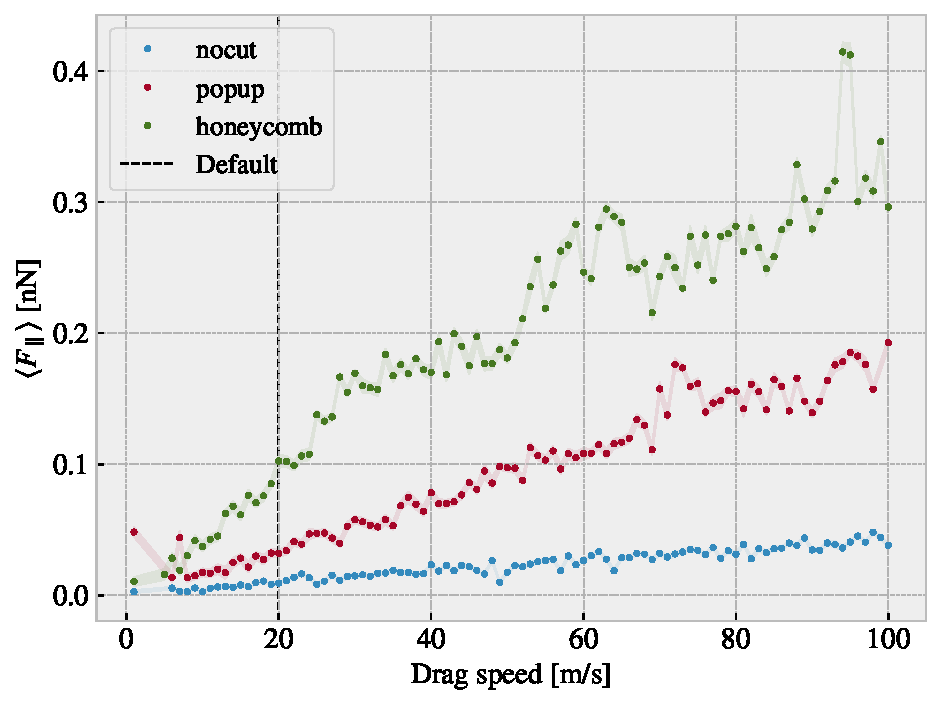
\includegraphics[width=\textwidth]{figures/baseline/variables_vel_mean_fixmove.pdf}
      \caption{Dynamic friction force estimate.}
      \label{fig:var_vel_mean}
  \end{subfigure}
  \hfill
  \begin{subfigure}[t]{0.49\textwidth}
      \centering
      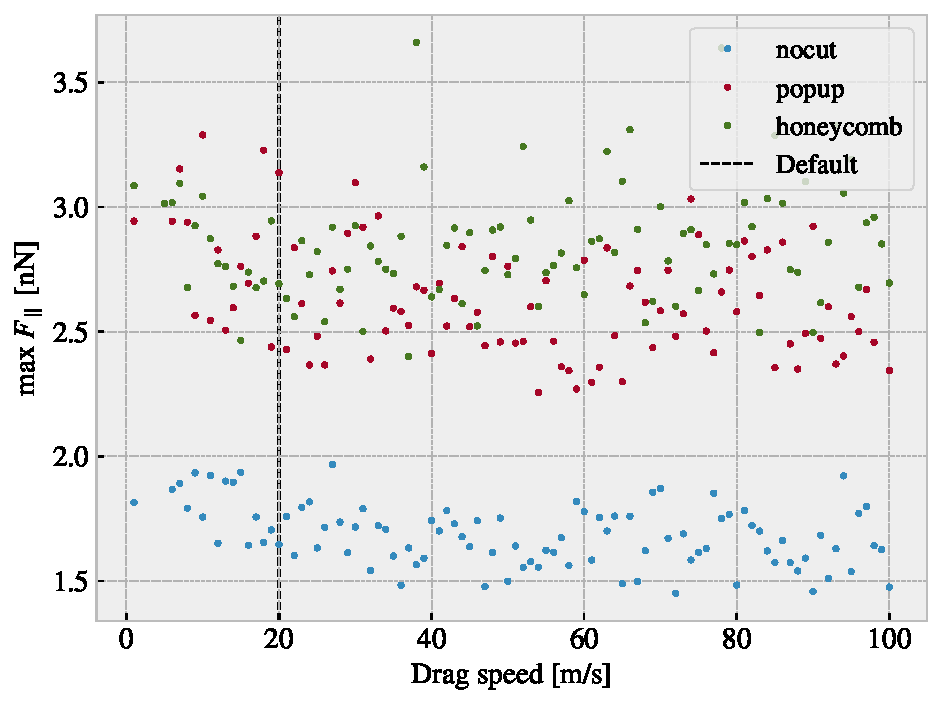
\includegraphics[width=\textwidth]{figures/baseline/variables_vel_max_fixmove.pdf}
      \caption{Max friction}
      \label{fig:var_vel_max}
  \end{subfigure}
  \hfill
     \caption{Sliding speed}
     \label{fig:var_vel}
\end{figure}



\begin{figure}[H]
  \centering
  \begin{subfigure}[t]{0.49\textwidth}
      \centering
      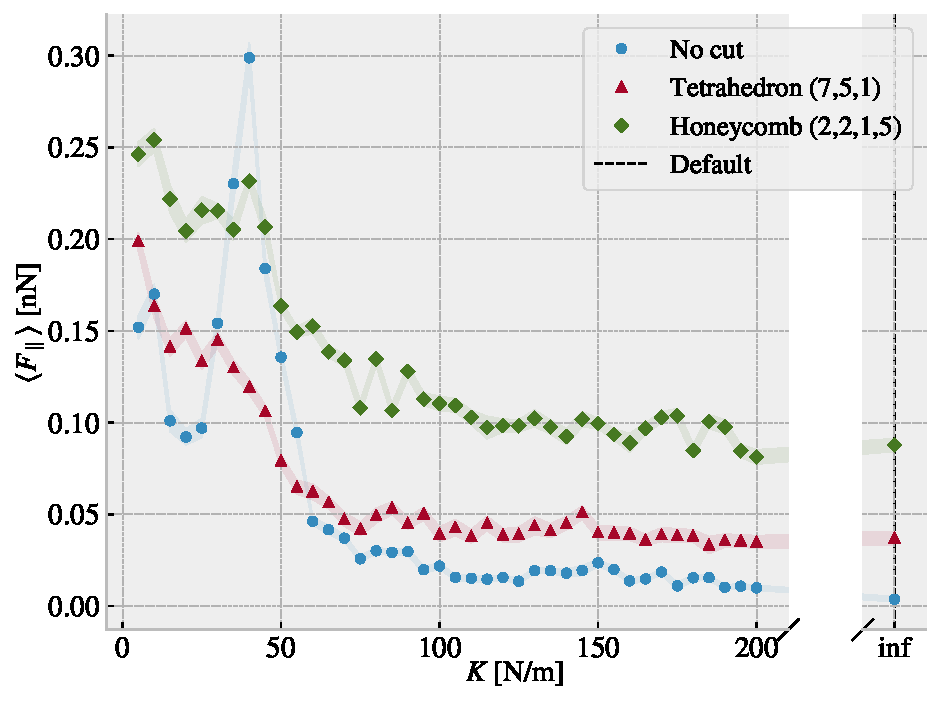
\includegraphics[width=\textwidth]{figures/baseline/variables_spring_mean_fixmove.pdf}
      \caption{Dynamic friction force estimate.}
      \label{fig:var_K_mean}
  \end{subfigure}
  \hfill
  \begin{subfigure}[t]{0.49\textwidth}
      \centering
      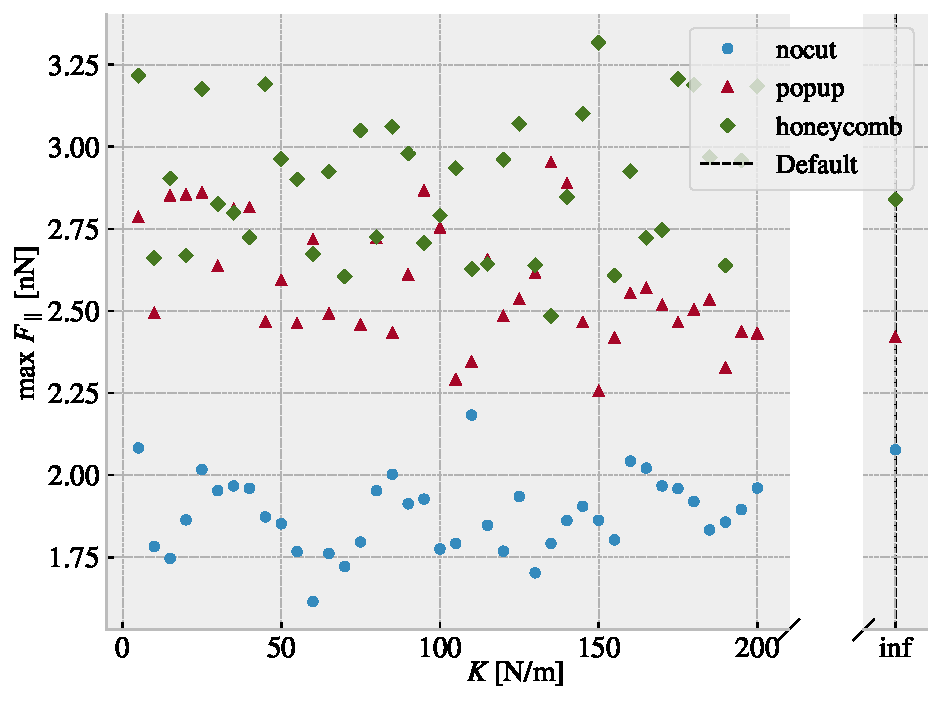
\includegraphics[width=\textwidth]{figures/baseline/variables_spring_max_fixmove.pdf}
      \caption{Max friction}
      \label{fig:var_K_max}
  \end{subfigure}
  \hfill
     \caption{Spring constant}
     \label{fig:var_K}
\end{figure}



\begin{figure}[H]
  \centering
  \begin{subfigure}[t]{0.49\textwidth}
      \centering
      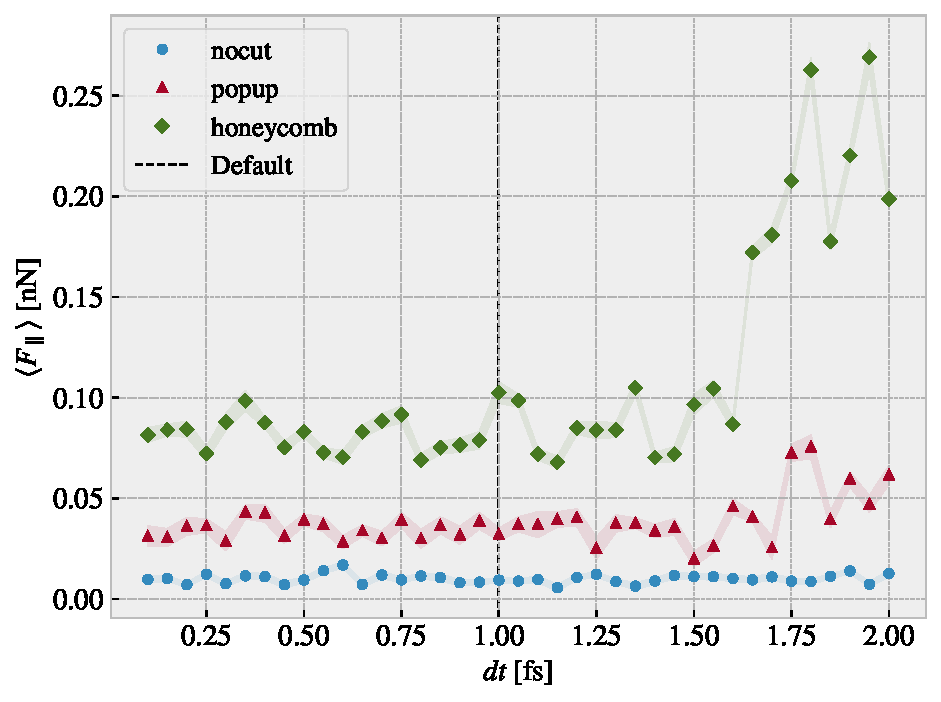
\includegraphics[width=\textwidth]{figures/baseline/variables_dt_mean_fixmove.pdf}
      \caption{Dynamic friction force estimate.}
      \label{fig:var_dt_mean}
  \end{subfigure}
  \hfill
  \begin{subfigure}[t]{0.49\textwidth}
      \centering
      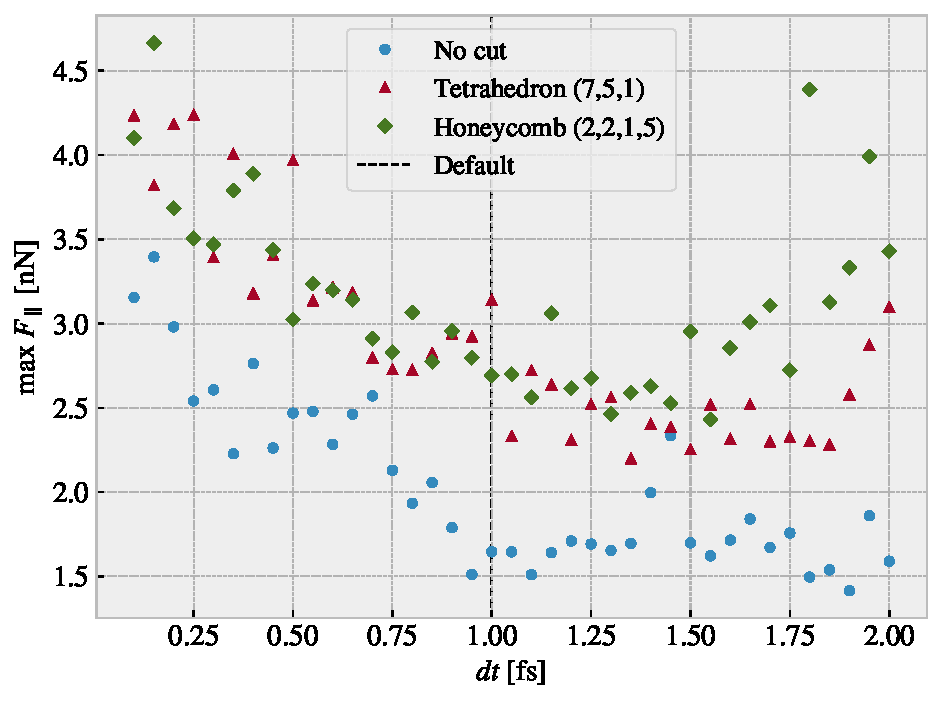
\includegraphics[width=\textwidth]{figures/baseline/variables_dt_max_fixmove.pdf}
      \caption{Max friction}
      \label{fig:var_dt_max}
  \end{subfigure}
  \hfill
     \caption{Timestep}
     \label{fig:var_dt}
\end{figure}


Quick thoughts:
\begin{itemize}
  \item Temperature: We do clearly not see the $1/T$ temperature decrease. The non-cut sheet seems to showcase a lienar relationship which is also somewaht present for the honeycomb which matches some of the findings in other MD simulations. For the popup we do see a local decrease at low temperatures which flip at around the default $T = \SI{300}{K}$ temperature. The max friction peaks seem to increase with temperatur as well indicating that the peaks might be associated with thermal fluctuations rather than actual stick-slip behaviour. This supports the finding that the static friction response is not significantly present in these simulations. 
  \item Velcotiy: Considering the non-cut sheet first the velocity dependency is seemingly linear which deviates from the expected logaritmic trend. For the cutted configurations we find some peaks which might indicate the presence of resonance frequencies. The cutted sheet might be closer to a logaritmic trend, but this is not spot on either. The max friction seems to decrease slightly with small velcoties and then stay rather constant. This can probably be explained by the reduced time to stick between stick slip. 
  \item Spring constant: On all three configurations the dynamic friction decreases with an increasing spring constant. The best explanations might be due to the lack of freedom to ``get stuck'' in incommensurable configurations. We also notice that the friction varies a lot at lower spring constants supporting the choice of having a stiff spring for stability reasons. Especially the non-cut sheet peaks at $K = \SI{40}{N/m}$. The max friction seem to be constant with $K$.
  \item $dt$: The dynamic friction is relatively stable around the default choice of $dt = \SI{1}{fs}$. However, the fluctuations with respect to $dt$ is more significant for popup pattern and even more for the honeycomb pattern. This indicates that the more complex dynamics of the simulation is more sensitive to the timestep. We might interpret this information as an additional measure of uncertainty. The maximum friction decreases with increasing timestep which can be asserted a statistical interpretation: Higher peaks will be captured by the high resolution of a low $dt$ and vice versa. The high max values towards the point of $dt = \SI{2}{fs}$ is most likely due to the approach of unstability in the simulation as seen more clearly for the dynamic friction evaluation. 
\end{itemize}


\subsection{Normal force and stretch dependencies}
Till this point we have only changed variables one by one to investigate single dependencies. We now advance the sutdy to a simultaneous variation of stretch and normal force.

\hl{Explain how the stretch is uniformly sampled within equally divided intervals and the normal force is actually uniformly sampled in a given range. Argue that the first might be approximately uniformly distributed for large numbers.}

\hl{Talk about rupture test also. Maybe in the theory/method section under numerical procedure: Before simulating a rupture test is perform to determine under what stretch the sheet ruptures. This is a slightly higher threshold than when applied normal load and sliding along the substrate.}

\subsubsection{Contact area}\ref{sec:contact_area}

We reproduce the contact area investigation of figure \ref{fig:contact_vs_stretch} with the modificaiton that the contact count is measured as an average of the latter 50\% of the sliding simulation at a non-zero applied normal load. The results are shown in figure \ref{fig:multi_stretch_contact} with 30 attempted (some rupture) stretch (pseudo) uniformly distributed stretch between 0 and the rupture point and 3 uniform distributed normal loads in the interval $[0.1, 10]$ nN. 


\begin{figure}[H]
  \centering
  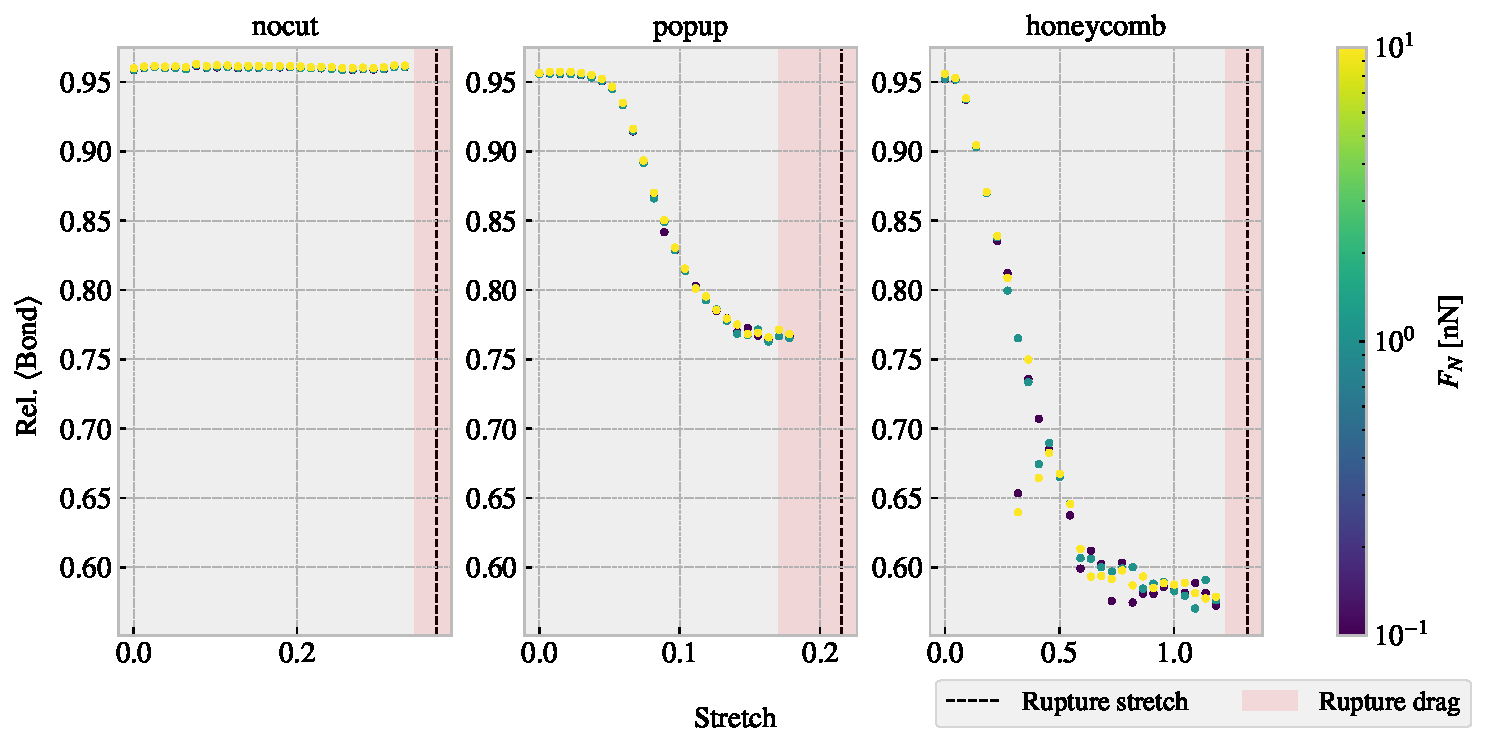
\includegraphics[width=\linewidth]{figures/baseline/multi_stretch_area_compare.pdf}
  \caption{Average relative amount of bonds beetwen the sheet and the substrate defined by the cut-off distance of 4 Å. The average is taken over the latter half of the sliding phase. The red shade denotes the stretch range where ruptures accour at certain normal loads under sliding while the black-dotted line represent the rupture point due to stretching (rupture test)}
  \label{fig:multi_stretch_contact}
\end{figure}

From figure \ref{fig:contact_vs_stretch} we observe a significant decrease in the contact due to stretching of the cut configurations in contrast to the non-cut which stays roughly constant. This is reminiscent of the non-sliding stretch vs. contact curve shown in figure \ref{fig:contact_vs_stretch}. Given these results, theoretically one would expect the dynamic friction to decrease with stretch for the cut configurations.


\subsubsection{Stretch} 

We make a similar analysis as done in the previous section \ref{sec:contact_area} with the substitution of friction force instead of contact (The data is taken from the same simulaitons runs). The dynamic friction force (\hl{put uncertainty here even though that it is quite low?}) and the max friction is shown in figure \ref{fig:multi_stretch_mean_fric} and \ref{fig:multi_stretch_max_fric} respectively.



\begin{figure}[H]
  \centering
  \begin{subfigure}[t]{\textwidth}
      \centering
      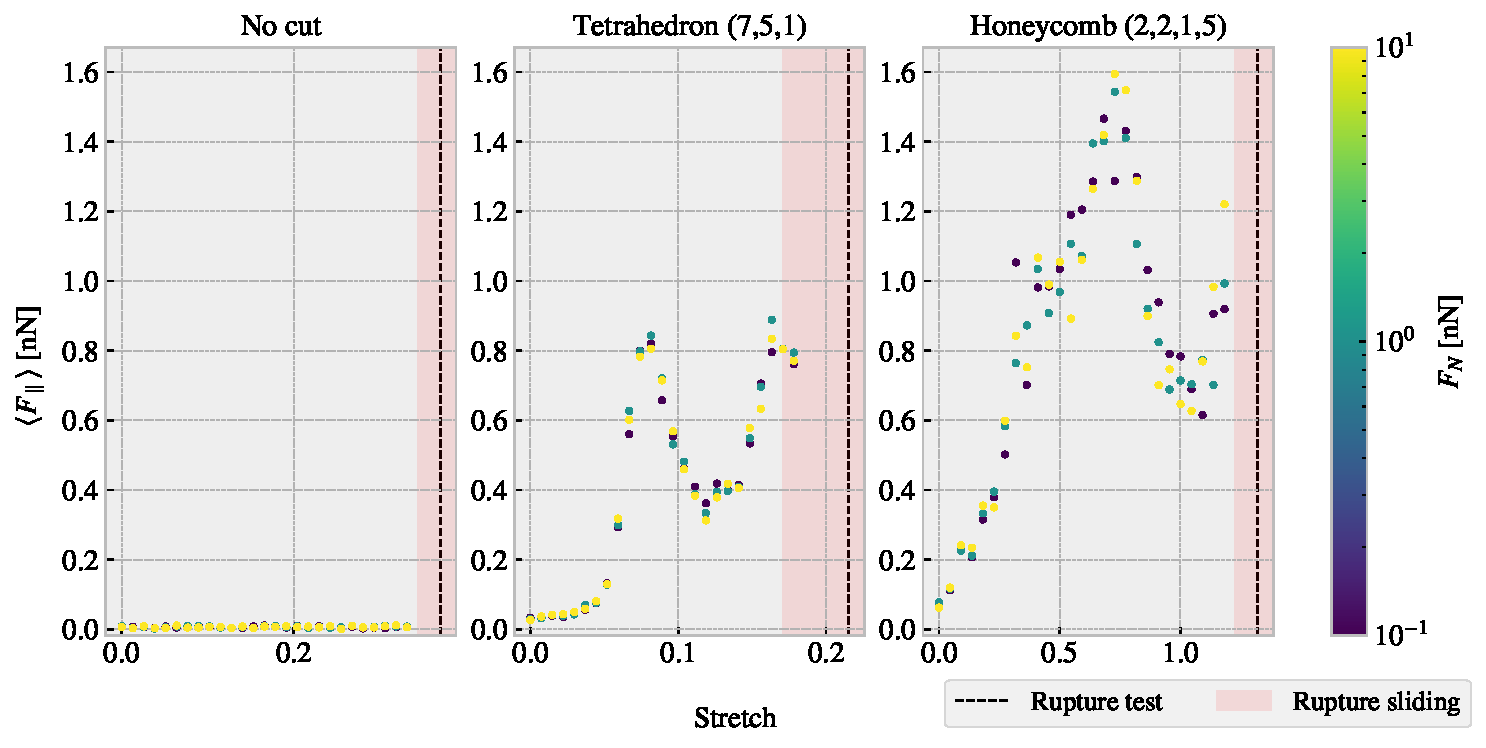
\includegraphics[width=\textwidth]{figures/baseline/multi_stretch_mean_compare.pdf}
      \caption{Dynamic friction estimate. }
      \label{fig:multi_stretch_mean_fric}
  \end{subfigure}
  \hfill
  \begin{subfigure}[t]{\textwidth}
      \centering
      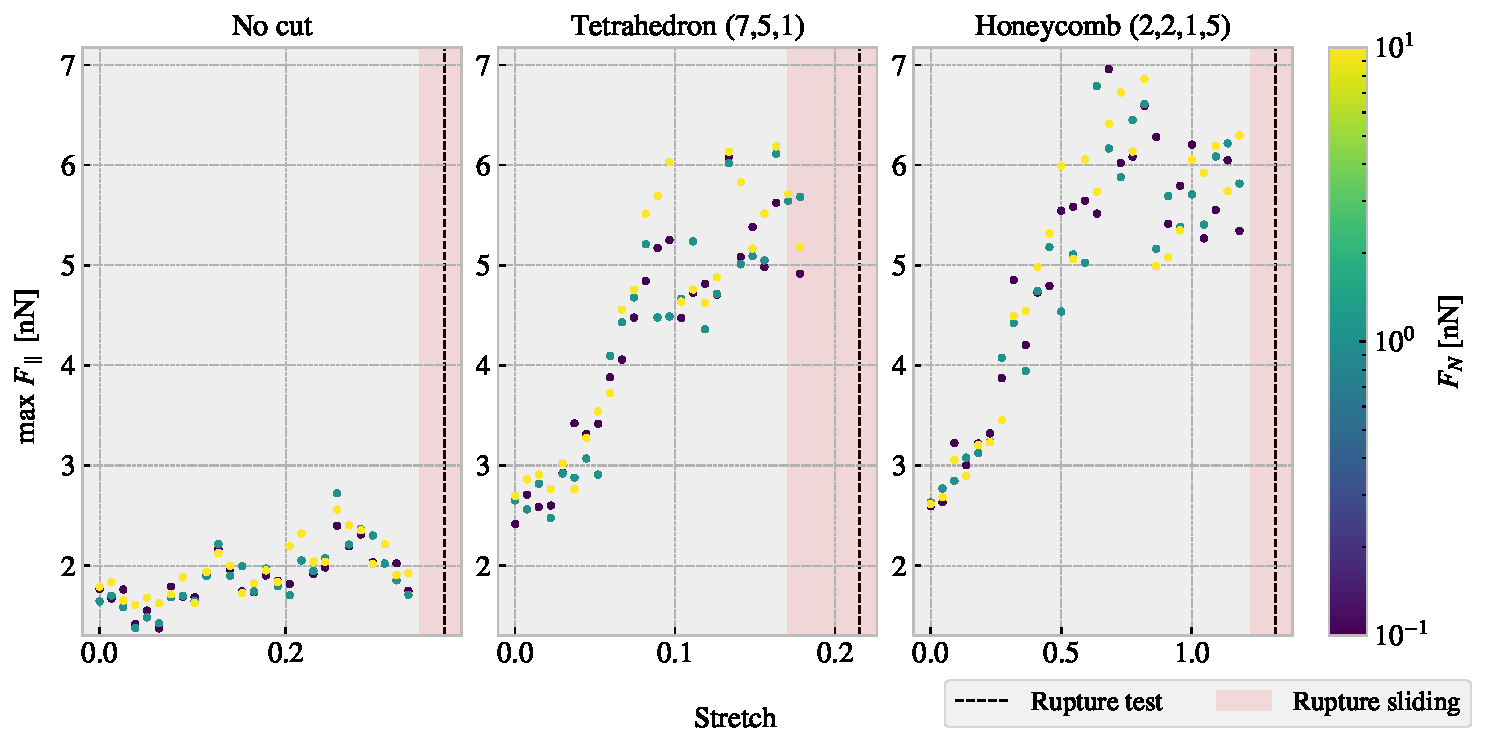
\includegraphics[width=\textwidth]{figures/baseline/multi_stretch_max_compare.pdf}
      \caption{Max friction}
      \label{fig:multi_stretch_max_fric}
  \end{subfigure}
  \hfill
     \caption{\hl{CAPTION}}
     \label{fig:multi_stretch_max_fric}
\end{figure}


From figure \ref{fig:multi_stretch_mean_fric} we find to our surprise that the
dynamic friction increase with stretch for the cut configurations despite a
simmutaneous decrease in contact area as shown in figure
\ref{fig:multi_stretch_contact}. This suggests that the amount of chemical
bonding atoms is not the dominant mechanism for the friction of this system.
Instead, we might point to a mechanism more mechanical of nature associated to
phonon exications. When the cut sheet is strecthed the stress (\hl{show stress
maps somewhere or not nessecary?}) might induce a certain distribution and
magnitude of point pressures to favor energy dissipation. Nonetheless, the
results showcase a strong coupling between stretch and friction force, also for
the max friction force, which is beyond the expectations at this stage of the
study. The non-cut configuration does not show significant dependency on the stretch which reveal that this effect is only present when combining cut and stretch and not purely by strecthing the sheet. 

By considering the increase in dynamic friction towards the first peak we get a relative friction increase and increase vs. stretch ratios as described in table \ref{tab:first_peak_stretch}. While the honeycomb force increase towards the first peak is approximately linear the popup exhibits seemingly exponential growth which yield a slope on the order $\sim \SI{30}{nN}$. 

\begin{table}[H]
  \begin{center}
  \caption{(stretch, dynamic friction) coordinates from figure \ref{fig:multi_stretch_mean_fric} at start and the first peak respectively used to approximate the relative increase in friction force and the ratio for friction increaese vs. stretch for sait range. In practice  the latter ratio denotes the slope of a forced linear trend. }
  \label{tab:first_peak_stretch}
  \begin{tabular}{ | c | c | c | c | c |} \hline
  Configuration & Start & First peak & Relative increase & Friction force vs. stretch ratio [nN]  \\ \hline
  Popup & $\sim (0, 0.03)$ & $\sim(0.082, 0.83)$ & 27.7 & 9.76  \\ \hline
  Honeycomb & $\sim (0, 0.07)$ &  $\sim (0.728, 1.57)$ & 22.4 & 2.06 \\ \hline
  \end{tabular}
  \end{center}
\end{table}

Additionally, we notice that booth the popup and honeycomb also exhibits stretch ranges where the dynamic friction force decrease with increasing stretch. Qualitatively we assign the slope to be on the same order of magnitude as those towrds the first peak. This is useful for the prospect of taking advantage of this phenonama as we can essentially achieve booth higher and lower friction for increasing stretch for different starting points. 


\subsubsection{Normal force}

\hl{Main take away from this section should be that the normal force does not really change the friction much; The friciton coefficient is extremely low, but I'm not sure how well the linear fits are (whether they are linear or sublinear). Not sure if I should do a linearly increasing normal force for better linear plots?}

\begin{figure}[H]
  \centering
  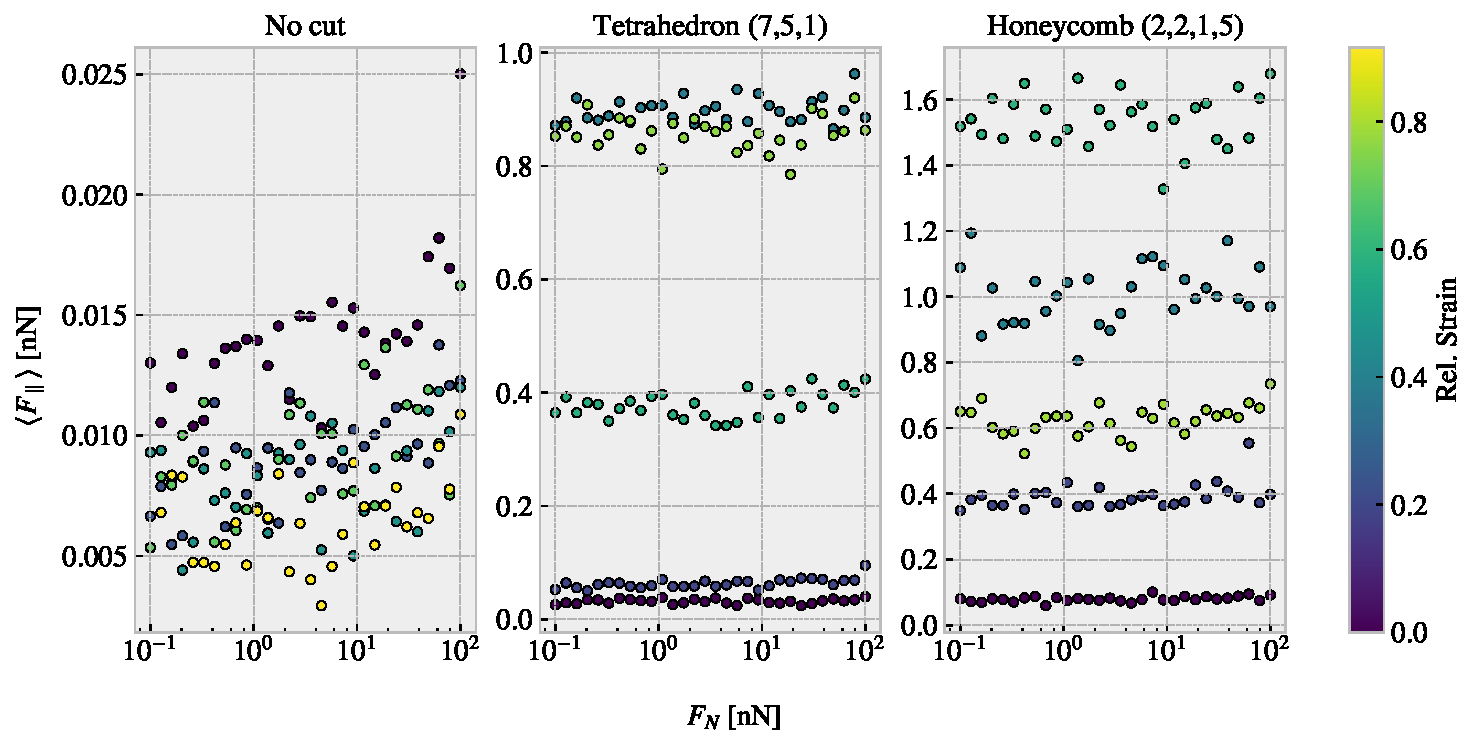
\includegraphics[width=\linewidth]{figures/baseline/multi_FN_mean_compare.pdf}
  \caption{...}
  \label{fig:}
\end{figure}


\begin{figure}[H]
  \centering
  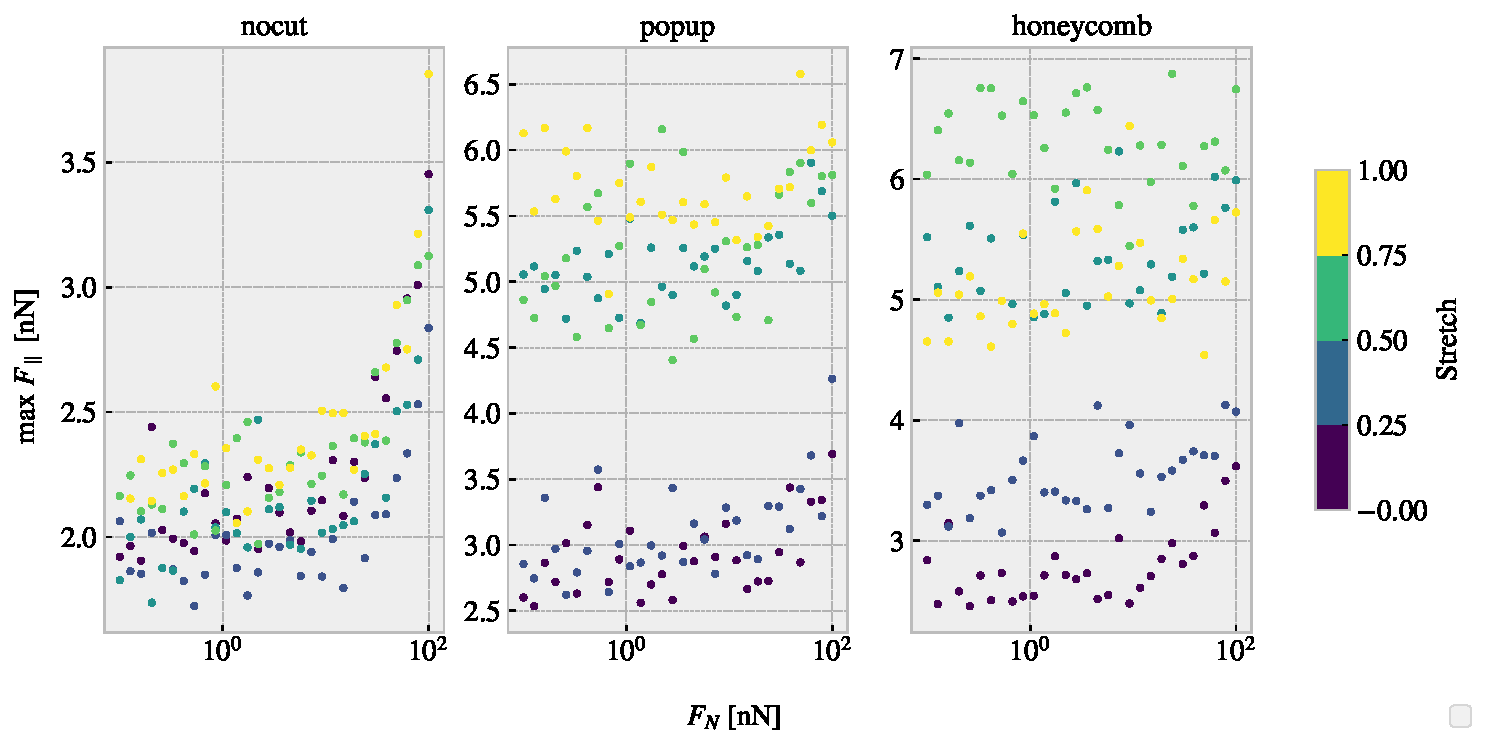
\includegraphics[width=\linewidth]{figures/baseline/multi_FN_max_compare.pdf}
  \caption{Colorbar is only fitted for the right plot (honeycomb)... this should be fixed. Should I have run a linear distribtion of FN so I could plot it linear here also...?}
  \label{fig:}
\end{figure}



\begin{table}[H]
  \begin{center}
  \caption{Mean friction coeff}
  \label{tab:fric_coeff}
  \begin{tabular}{| c | c | c | c | c | c |} \hline
    nocut & 0.00009 $\pm\num{1e-05}$ & 0.00005 $\pm\num{1e-05}$ & 0.00004 $\pm\num{1e-05}$ & 0.00005 $\pm\num{2e-05}$ & \\ \hline
    popup & 0.00005 $\pm\num{3e-05}$ & 0.00024 $\pm\num{5e-05}$ & 0.0002 $\pm\num{2e-04}$ & 0.0005 $\pm\num{1e-04}$ & 0.0003 $\pm\num{2e-04}$ \\ \hline
    honeycomb & 0.00013 $\pm\num{6e-05}$ & 0.0006 $\pm\num{3e-04}$ & 0.0004 $\pm\num{6e-04}$ & 0.0007 $\pm\num{6e-04}$ & 0.0009 $\pm\num{3e-04}$ \\ \hline
  \end{tabular}
  \end{center}
\end{table}

\begin{table}[H]
  \begin{center}
  \caption{Max friciton coeff}
  \label{tab:fric_coeff}
  \begin{tabular}{| c | c | c | c | c | c |} \hline
    nocut & $0.0139 \pm \num{9e-04}$& $0.0083 \pm \num{7e-04}$& $0.010 \pm \num{1e-03}$& $0.0105 \pm \num{9e-04}$ &  \\ \hline
    popup & $0.007 \pm \num{2e-03}$& $0.010 \pm \num{2e-03}$& $0.007 \pm \num{2e-03}$& $0.009 \pm \num{3e-03}$& $0.006 \pm \num{2e-03}$ \\ \hline
    honeycomb & $0.010 \pm \num{1e-03}$& $0.007 \pm \num{2e-03}$& $0.007 \pm \num{3e-03}$& $0.000 \pm \num{3e-03}$& $0.004 \pm \num{3e-03}$ \\ \hline
  \end{tabular}
  \end{center}
\end{table}


\hl{One theory for the low friction coefficient might dependent on the fact that the normal force is only applied on the pull blocks. Especially with the cutted sheet the tension drops such that the effecive normal force on the inner sheet is not changing very much. By this theory the friction force vs. normal force on the pull blocks should look a bit more like expected and we might make some plots of thoose to check}

\hl{When looking at the graphs for the PB the max friction is visually textbook linear, while the mean friction is a bit more linear but also with negativ coefficients...}



\subsection{Computational cost}

Talk about the computatonal cost of different choices. How does computation time scale with drag speed, $dt$ and maybe $T$ and $K$ as well. One could also mention scaling with system size.

Show how the number of cores per simulation scale to argue that running on just one core (maybe 4) is smart for the next step of many simulations. 

Mention the trouble with GPU to show that this was considered, and in fact this was the reason for choosing the Tersoff potential over the AIREBO which is perhaps more common these days...



\section{Generating data}

Present the configuration and variable choices for the generated dataset. Perhaps include appendix with all the configurations shown in a grid


\section{Training forward network}

\section{Inverse design}

\section{Negative friction coefficient}
\subsection{Simulated coupling of normal force and stretch}
\subsection{Nanomachine coupling}
Attempt to couple normal force and stretch by crossed carbon nanotube (CNT) contraption \ref{fig:nanomachine}. 


\begin{figure}[H]
  \centering
  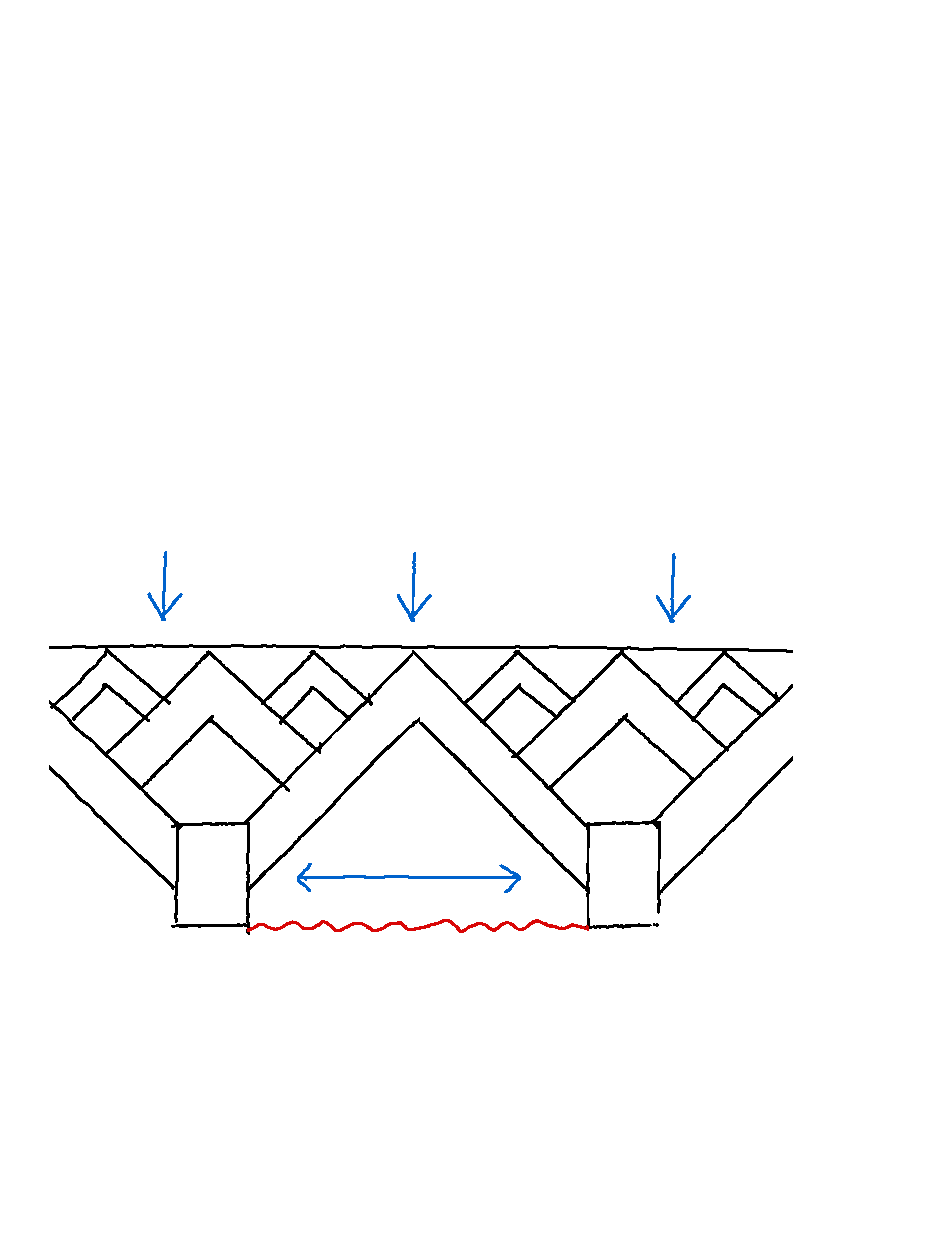
\includegraphics[width=0.5\linewidth]{figures/negative_coefficient/nanomachine.pdf}
  \caption{Working sketch for nanomachine}
  \label{fig:nanomachine}
\end{figure}



